\documentclass[xcolor=dvipsnames]{beamer}
\usepackage[T1]{fontenc}
\usepackage[utf8]{inputenc}
\usepackage[english,slovak]{babel}

\usepackage{amsmath}
\usepackage{amsthm}
\usetheme{Pittsburgh}
\useoutertheme{shadow}

\usepackage{graphicx}
\usepackage{caption}
\usepackage{subcaption}

\usepackage{tabularx}


\usepackage{listings}
\lstloadlanguages{Ruby}
\lstset{%
basicstyle=\ttfamily\color{black},
commentstyle = \ttfamily\color{red},
keywordstyle=\ttfamily\color{blue},
stringstyle=\color{orange}}



%-------------------------------------------------------------------------------------
\title{\bf Q-learning - umelá inteligencia na obzore?}
\author{Ing. Michal CHOVANEC \\Fakulta riadenia a informatiky}

\date[EURP]{\it Apríl 2016}
\begin{document}

\begin{frame}
\titlepage
\end{frame}


%“a way of programming agents by reward and
%punishment without needing to specify how the
%task is to be achieved”
%[Kaelbling, Littman, & Moore, 96]


%-------------------------------------------------------------------------------------
\begin{frame}{\bf Obsah}

\begin{minipage}{.5\textwidth}

\begin{itemize}
  \item Reinforcement learing
  \item Q-learning algoritmus
  \item Možnosti aproximácie
\end{itemize}

  \end{minipage}%
\begin{minipage}{.5\textwidth}

  \begin{figure}[!htb]
  \centering
  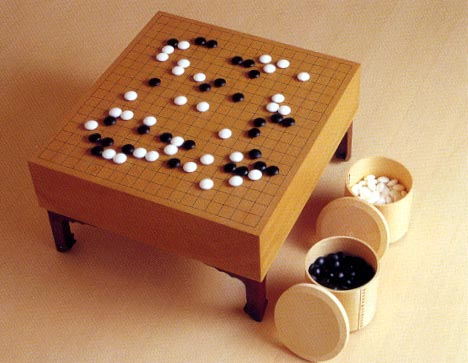
\includegraphics[scale=.8]{../pictures/go.jpg}
  \end{figure}

\end{minipage}

\end{frame}


%-------------------------------------------------------------------------------------
\begin{frame}{\bf Reinforcement learing}

\begin{minipage}{.5\textwidth}

\begin{itemize}
  \item Zistenie stavu
  \item Výber akcie
  \item Vykonanie akcie
  \item Prechod do ďalšieho stavu
  \item Získanie odmeny alebo trestu
  \item Učenie sa zo získanej skúsenosti
\end{itemize}

  \end{minipage}%
\begin{minipage}{.5\textwidth}

  \begin{figure}[!htb]
  \centering
  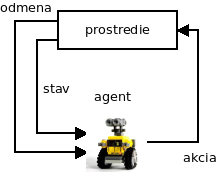
\includegraphics[scale=.8]{../diagrams/agent.png}
  \end{figure}

\end{minipage}

\end{frame}

\begin{frame}{\bf Výhody}

Definuje sa čo robiť, nie ako to robiť
\begin{itemize}
\item vďaka odmeňovacej funkcií
\item agent sa môže naučiť všetky detaily problému
\end{itemize}

Lepšie konečné riešenie
\begin{itemize}
\item založené na skutočnej skúsenosti, nie skúsenosti programátora
\item treba menej ľudského času na nájdenie dobrého riešenia
\end{itemize}


\end{frame}


%-------------------------------------------------------------------------------------
\begin{frame}{\bf Voľba stratégie, 2 stavy}

  Odmeny sú známe v každom prechode

  \begin{figure}[!htb]
  \centering
  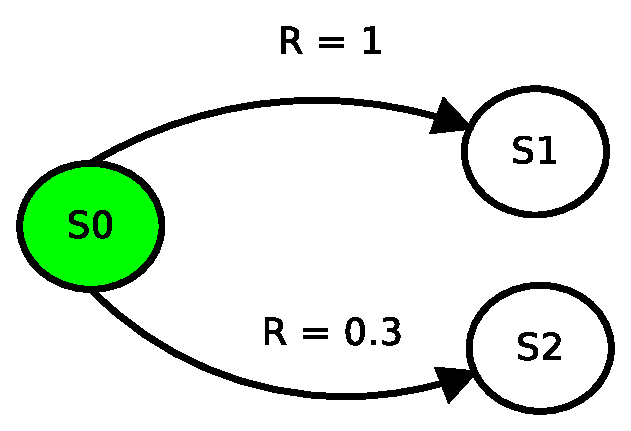
\includegraphics[scale=.6]{../diagrams/rf_two_states.eps}
  \end{figure}

  Ohodnotenie ciest :
  \begin{itemize}
    \item $Q(S0, S1) = 1$
    \item $Q(S0, S1) = 0.3$
  \end{itemize}

  Najlepšia cesta : $S0, S1$
\end{frame}


%-------------------------------------------------------------------------------------
\begin{frame}{\bf Voľba stratégie, viac stavov}

  \begin{figure}[!htb]
  \centering
  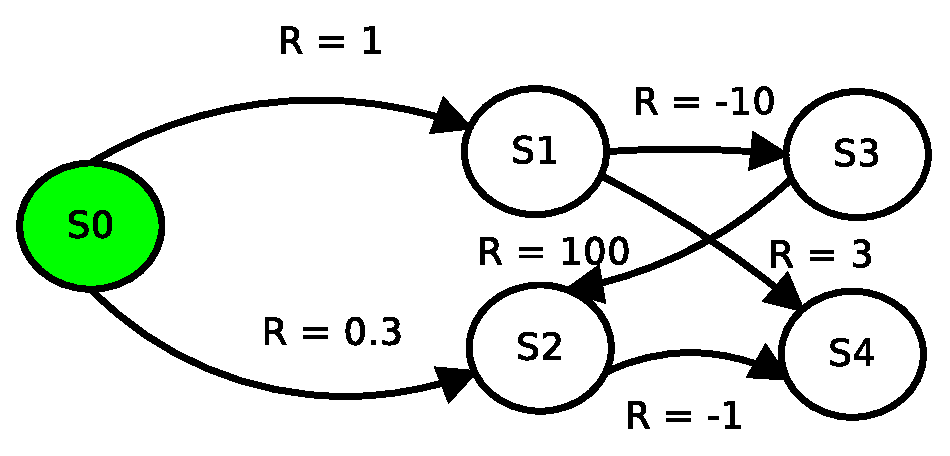
\includegraphics[scale=.6]{../diagrams/rf_more_states.eps}
  \end{figure}

  Ohodnotenie ciest :
  \begin{itemize}
    \item $Q(S0, S1, S3) = 1+(-10) = -9$
    \item $Q(S0, S1, S4) = 1+3 = 4$
    \item $Q(S0, S2, S4) = 0.3 +()-1) =-0.7$
    \item $Q(S0, S1, S3, S2, S4) = 1 +(-10) +100 + (-1) = 90$
    \item ...
  \end{itemize}

\end{frame}

%-------------------------------------------------------------------------------------
\begin{frame}{\bf Voľba stratégie, viac stavov}

  \begin{figure}[!htb]
  \centering
  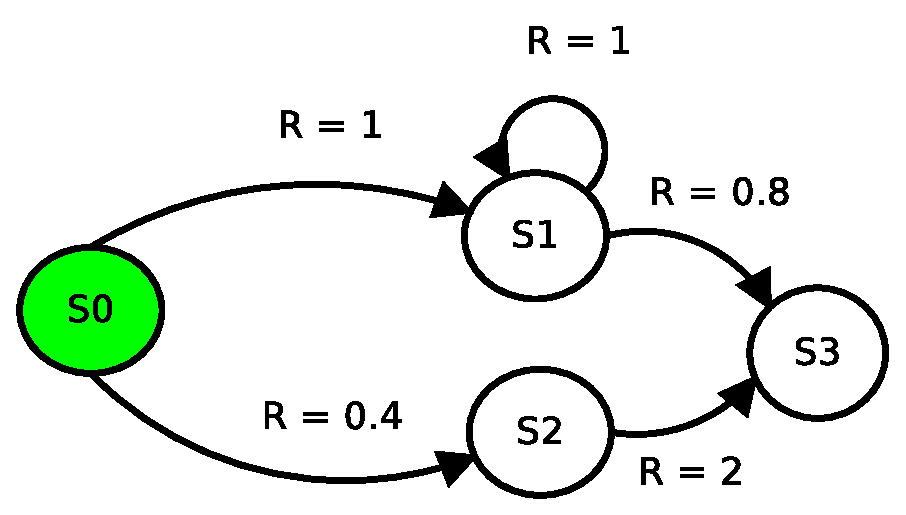
\includegraphics[scale=.6]{../diagrams/rf_cycle_states.eps}
  \end{figure}

  Ohodnotenie ciest :
  \begin{itemize}
    \item $Q(S0, S2, S3) = 0.4+2 = 2.4$
    \item $Q(S0, S1, S3) = 1+1 = 2$
    \item $Q(S0, S1, S1, S1) = 1+1+1 = 3$
    \item $Q(S0, S1, S1, S1, S1) = 1+1+1+1 = 4$
    \item $Q(S0, S1, S1, S1, S1, S1, ...) = 1+1+1+1+1+...+1 = \infty$ !!!!
  \end{itemize}

\end{frame}


%-------------------------------------------------------------------------------------
\begin{frame}{\bf Zabúdanie   $Q' = R + 0.9Q$}

  \begin{figure}[!htb]
  \centering
  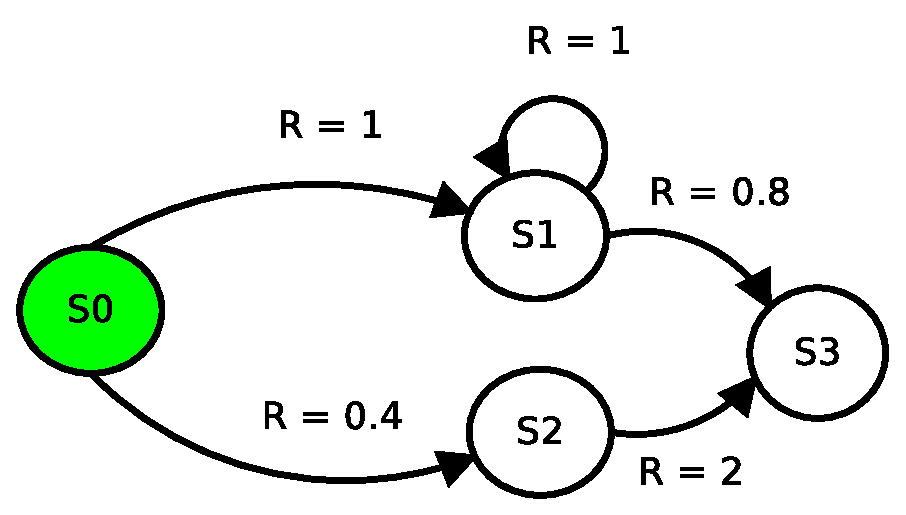
\includegraphics[scale=.5]{../diagrams/rf_cycle_states.eps}
  \end{figure}

  Ohodnotenie ciest :
  \begin{itemize}
    \item $Q(S0, S2, S3) = 2 + 0.9*0.4 = 2.36$
    \item $Q(S0, S1, S3) = 1 + 0.9*1 = 1.9$
    \item $Q(S0, S1, S1, S1) = 1 + 0.9*(1 + 0.9*1) = 2.71 $
    \item $Q(S0, S1, S1, S1, S1) = 1 + 0.9*(1 + 0.9*(1 + 0.9*1)) = 3.439$
    \item $Q(S0, S1, S1, S1, S1, S1, ...) = 10$ <-----
    \item $Q(S0, S1, S1, S1, S1, S1, ..., S3) = 11$ <-----
  \end{itemize}

\end{frame}


%-------------------------------------------------------------------------------------
\begin{frame}{\bf Reinforcement learing}

Čo ak odmeny NIE sú známe v každom prechode ?

\begin{itemize}
  \item šachy, go, pacman
  \item chôdza, pohyb mechanického ramena
\end{itemize}

\end{frame}


%-------------------------------------------------------------------------------------
\begin{frame}{\bf Reinforcement learing}

\begin{minipage}{.5\textwidth}
Čo potrebuje agent?
\begin{itemize}
  \item Určiť stav
  \item Vybrať známu akciu
  \item Dostať odmenu (aj nulovú)
  \item Pamätať si
\end{itemize}

  \end{minipage}%
\begin{minipage}{.5\textwidth}
  Čo nepotrebuje agent?

  \begin{itemize}
    \item Dané správanie
    \item Vedieť kam sa vykonaním akcie dostane
    \item Mať model prostredia
    \item Nenulovú odmenu v každom prechode
  \end{itemize}

\end{minipage}


\end{frame}



%-------------------------------------------------------------------------------------
\begin{frame}{\bf Ilustračný príklad - inicializácia}

\begin{figure}[!htb]
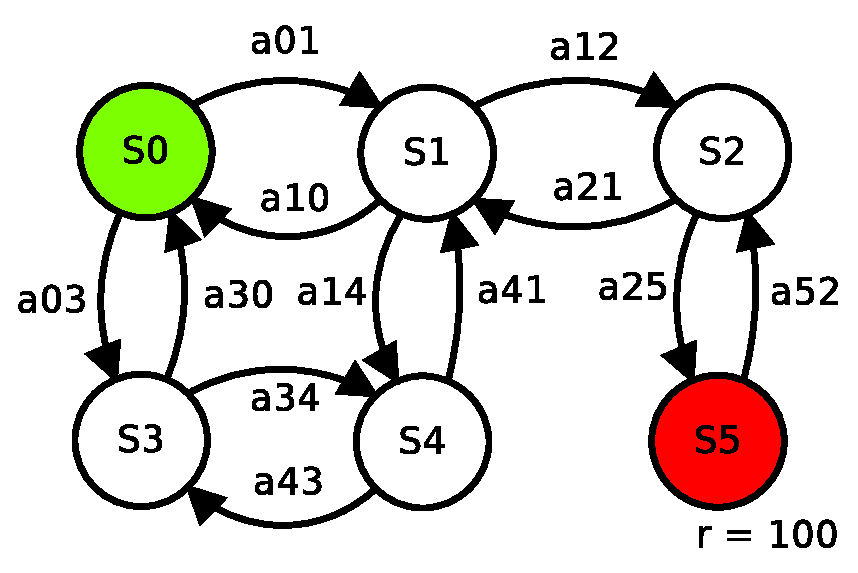
\includegraphics[scale=.5]{../diagrams/q_learning_table_01.eps}
\end{figure}

\end{frame}

%-------------------------------------------------------------------------------------
\begin{frame}{\bf Ilustračný príklad - prechod do ďalšieho stavu}

\begin{figure}[!htb]
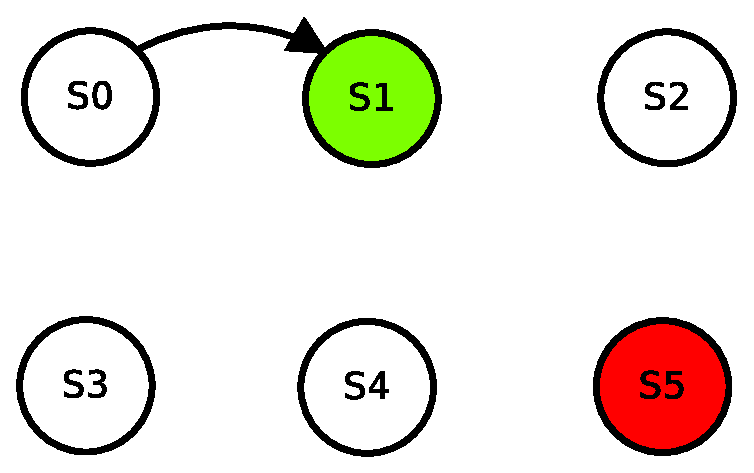
\includegraphics[scale=.5]{../diagrams/q_learning_table_02.eps}
\end{figure}

\end{frame}

%-------------------------------------------------------------------------------------
\begin{frame}{\bf Ilustračný príklad - prechod do ďalšieho stavu}

\begin{figure}[!htb]
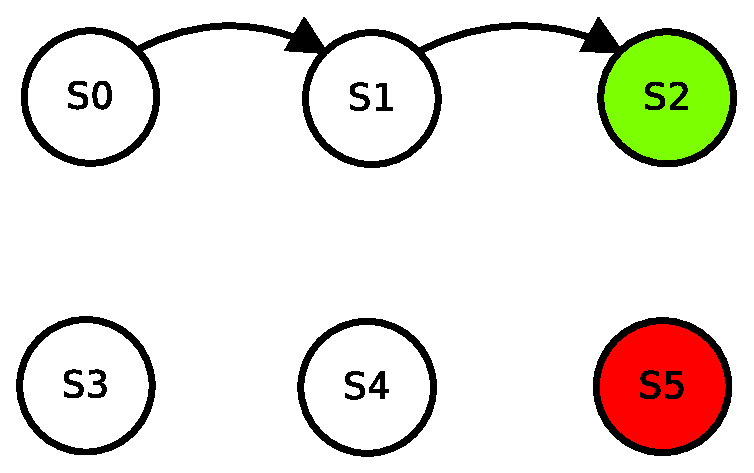
\includegraphics[scale=.5]{../diagrams/q_learning_table_03.eps}
\end{figure}

\end{frame}

%-------------------------------------------------------------------------------------
\begin{frame}{\bf Ilustračný príklad - prechod do cieľového stavu}

\begin{figure}[!htb]
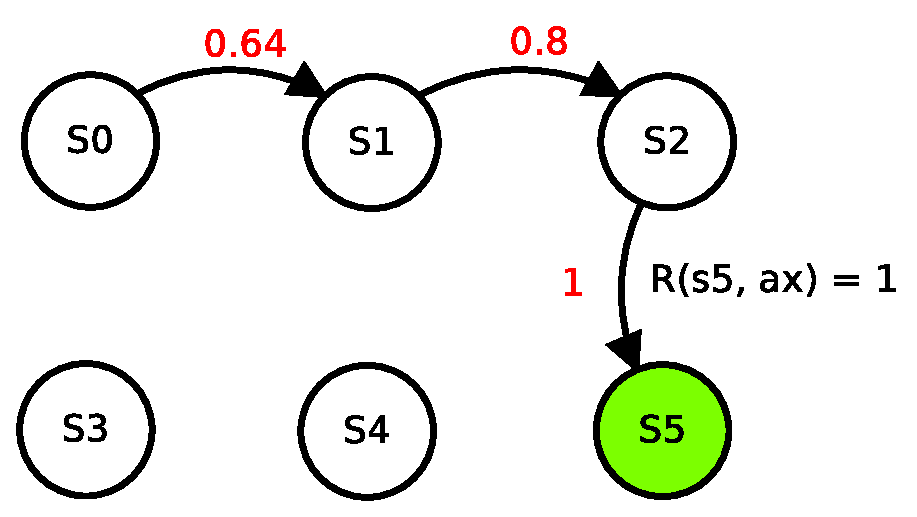
\includegraphics[scale=.5]{../diagrams/q_learning_table_04.eps}
\end{figure}

\end{frame}

%-------------------------------------------------------------------------------------
\begin{frame}{\bf Ilustračný príklad - ďalšie prechody}

\begin{figure}[!htb]
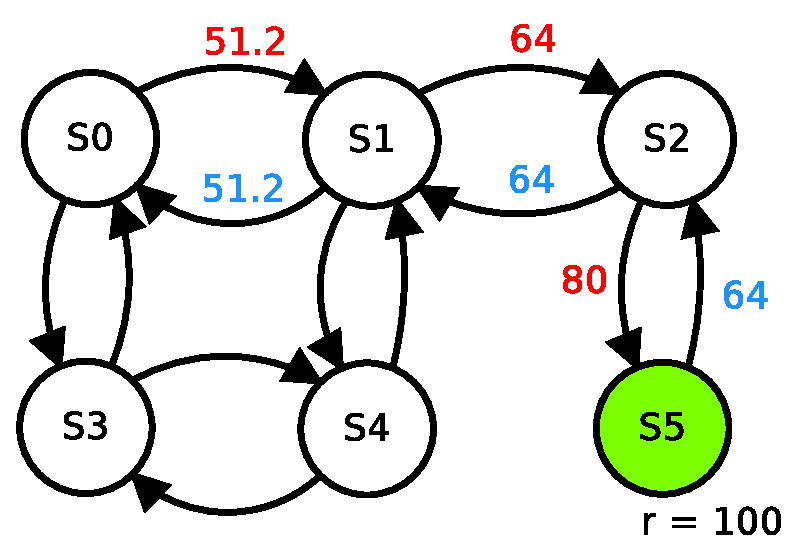
\includegraphics[scale=.5]{../diagrams/q_learning_table_05.eps}
\end{figure}

\end{frame}

%-------------------------------------------------------------------------------------
\begin{frame}{\bf Ilustračný príklad - konečný stav algoritmu :)}

\begin{figure}[!htb]
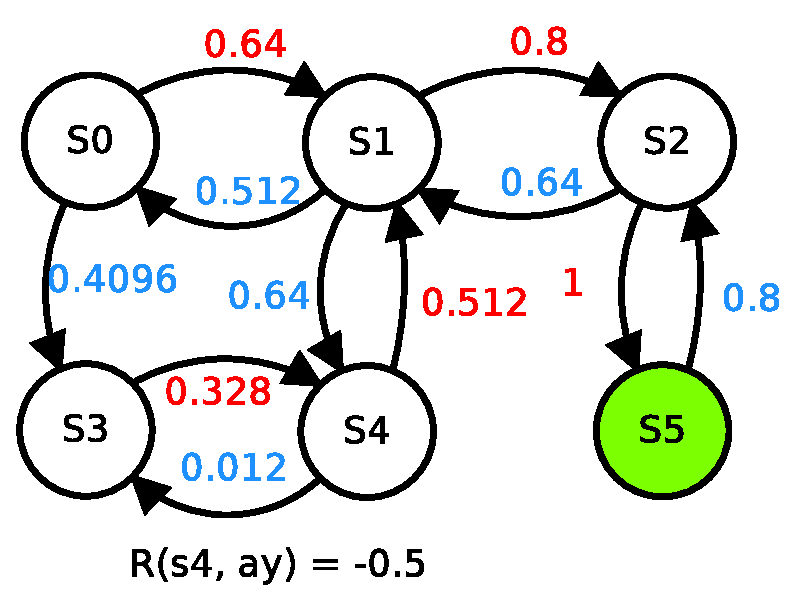
\includegraphics[scale=.5]{../diagrams/q_learning_table_06.eps}
\end{figure}

\end{frame}



%-------------------------------------------------------------------------------------
\begin{frame}{\bf Q-learning algoritmus}

Daná je množina stavov $\mathbb{S}$ a akcií $\mathbb{A}$, kde
 $\mathbb{S} \in \mathbb{R}^{n_s}$ a $\mathbb{A} \in \mathbb{R}^{n_a}$, kde
$n_s$ a  $n_a$ sú rozmery stavového vektora a vektora akcií. Je známa podmnožina východiskových
stavov $\mathbb{S}_0$.

Existuje prechodová funkcia
\begin{align}
        s(n+1) = \lambda(s(n), a(n))
\end{align}
zo stavu $s(n)$ použitím akcie $a(n)$ - táto funkcia je ale agentovi neznáma.


%Cieľom je nájsť takú postupnosť akcií $a(i) \in \mathbb{A}$ z východiskového stavu $s(0) \in \mathbb{S}_0$ pre ktorú bude maximálne

%\begin{equation} \label{eu_eqn}
%y({s(0)}) = \prod_{i=0}^{t}Q(s(i), a(i)) ,
%\end{equation}

%kde $s(t)$ je cieľový stav a $Q(s(i), a(i))$ je funkcia ohodnotení akcie $a(i)$ v stave
%$s(i)$.



\end{frame}



%-------------------------------------------------------------------------------------
\begin{frame}{\bf Odmeňovacia funkcia}

Daná je funkcia ohodnotení

\begin{equation}
Q(s(n),a(n)) = R(s(n),a(n)) + \gamma \max_{a(n-1) \in \mathbb{A}} Q(s(n-1), a(n-1)) \nonumber
\end{equation}

kde \\

\begin{itemize}
 \item $R(s(n),a(n))$ je odmeňovacia funkcia s hodnotami v $\langle -1, 1 \rangle$, \\
 \item $Q(s(n-1),a(n-1))$ je odmeňovacia funkcia v stave $s(n-1)$ pre akciu $a(n-1)$, \\
 \item $\gamma$ je odmeňovacia konštanta a platí $\gamma \in (0, 1)$.
\end{itemize}

\end{frame}


%-------------------------------------------------------------------------------------
\begin{frame}{\bf Odmeňovacia funkcia}

\begin{figure}[!htb]
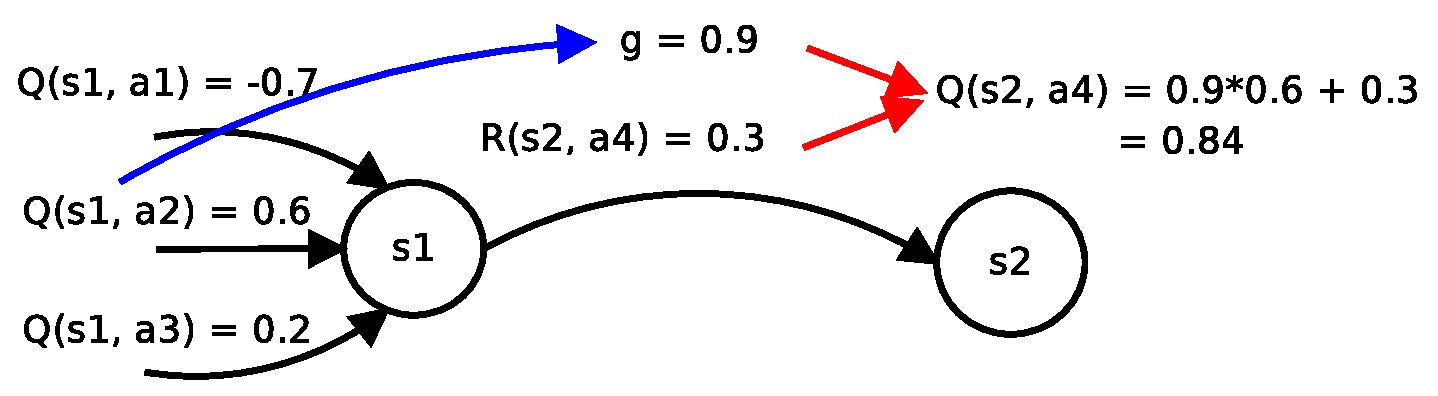
\includegraphics[scale=.4]{../diagrams/q_learning_detail.eps}
\end{figure}


\end{frame}



%-------------------------------------------------------------------------------------
\begin{frame}{\bf Implementačné problémy}

Problémy tabuľkovej interpretácie $Q(s(n), a(n))$ :

\begin{itemize}
\item pre veľké ${n_s}$  alebo  ${n_a}$ narastajú pamäťové nároky,
\item o nevyplnených $Q(s(n), a(n))$ nevieme povedať nič,
\item pre rozsiahle stavové priestory ťažko vypočítateľné,
\item ako aproximovať $Q(s(n), a(n))$?
\end{itemize}

\end{frame}


%-------------------------------------------------------------------------------------
\begin{frame}{\bf Aproximácia neurónovou sieťou}

Utopická predstava :

\begin{figure}[!htb]
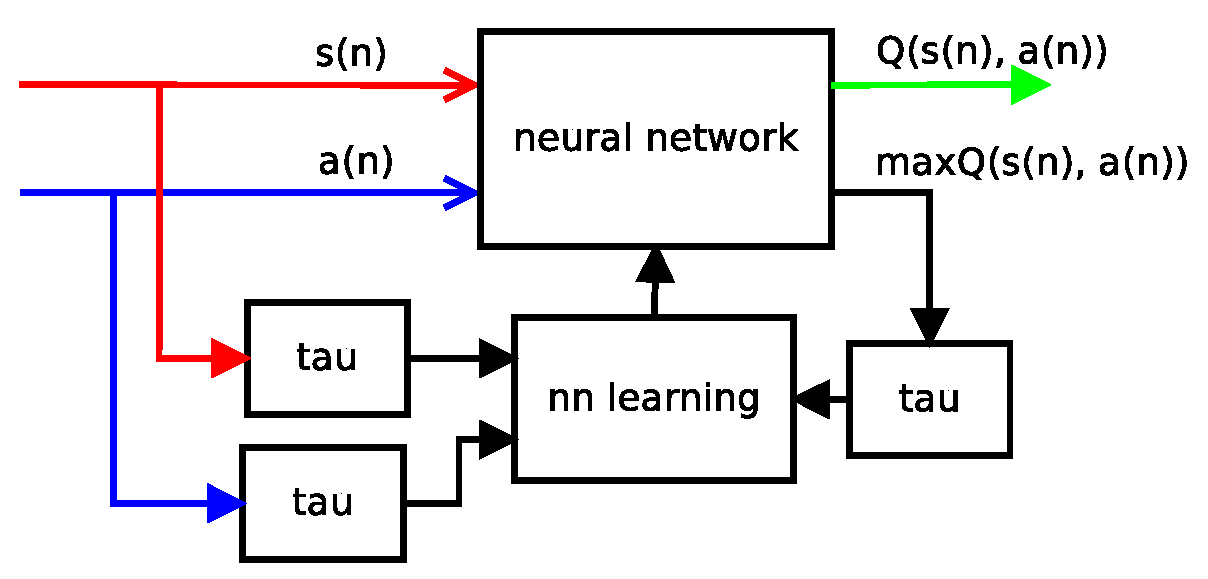
\includegraphics[scale=.5]{../diagrams/q_learning_nn.eps}
\end{figure}

Prečo nedáva správne výsledky?
\end{frame}


%-------------------------------------------------------------------------------------
\begin{frame}{\bf Hypotéza}

Na základe experimetov - Snowball problém

\begin{figure}[!htb]
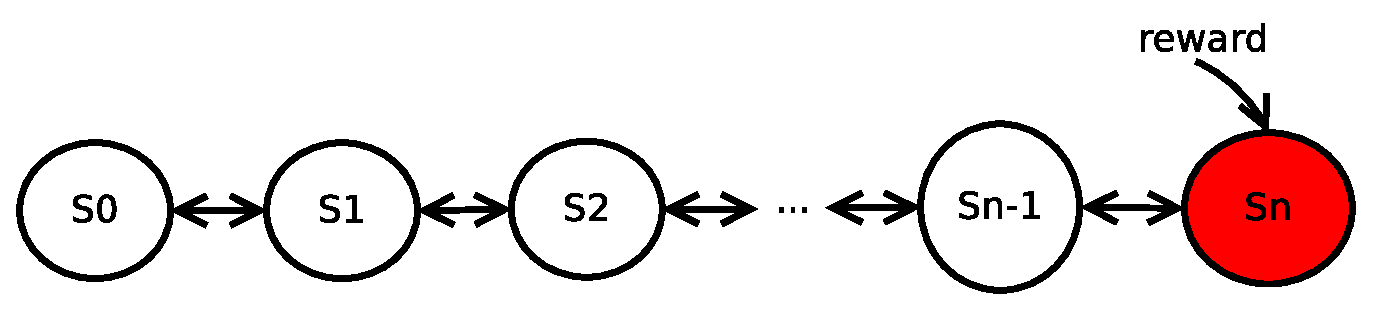
\includegraphics[scale=.5]{../diagrams/q_chain_problem.eps}
\end{figure}

Pre korektné vyplnenie hodnôt v $s_{n-1}$ sa vyžaduje korektá hodnota v $s_{n}$

\begin{align*}
    Q(s(1),a(1)) &= R(s(1),a(1)) + \gamma \max_{a(0) \in \mathbb{A}} Q(s(0), a(0)) \\
    Q(s(2),a(2)) &= R(s(2),a(2)) + \gamma \max_{a(1) \in \mathbb{A}} Q(s(1), a(1)) \\
    & \dots
\end{align*}

\end{frame}



%-------------------------------------------------------------------------------------
\begin{frame}{\bf Učenie doprednej siete}

\begin{itemize}
 \item Nie je homogénne! \\
 \item V priebehu učenia $Q(s(n),a(n))$ chaoticky osciluje okolo požadovanej hodnoty. \\
 \item Ani po 10-mil. iteráciach sa hodnota neustáli na požadovanej hodnote.
\end{itemize}

\end{frame}


%-------------------------------------------------------------------------------------
\begin{frame}{\bf Je možné zostaviť neurónovú sieť, ktorá sa dá naučiť lokálne?}

\begin{figure}[!htb]
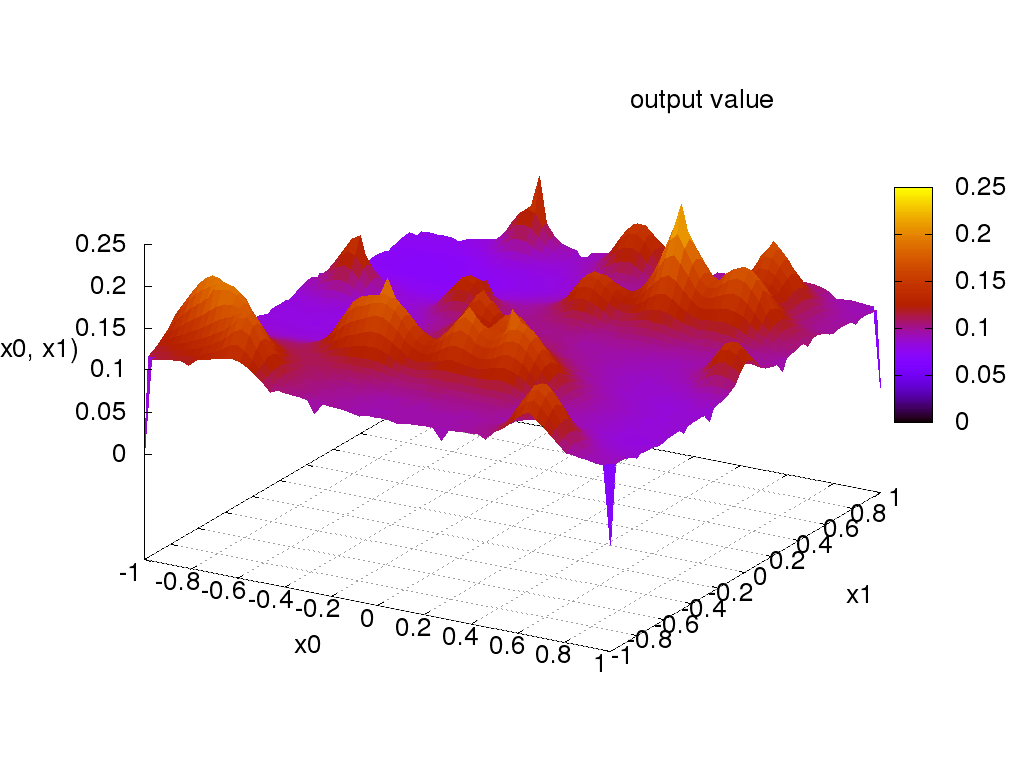
\includegraphics[scale=.35]{../pictures/gaussian.png}
\end{figure}

\end{frame}


%-------------------------------------------------------------------------------------
\begin{frame}{\bf Rozklad $Q(s(n), a(n))$ na bázické funkcie}


\begin{align*}
    f_j^1(\boldmath{s(n), a(n)}) &= e^{ -\sum\limits_{i=1}^{n_s}{\beta_{aji}(n)(s_i(n) - \alpha_{aji}(n))^2} } \nonumber \\
    \\
    f_j^2(\boldmath{s(n), a(n)}) &= \frac{1}{1 + \sum\limits_{i=1}^{n_s}{\beta_{aji}(n)(s_i(n) - \alpha_{aji}(n))^2}} \nonumber \\
    \\
    f_j^3(\boldmath{s(n), a(n)}) &= e^{ -\sum\limits_{i=1}^{n_s}{\beta_{aji}(n)\mid s_i(n) - \alpha_{aji}(n) \mid} } \nonumber  \\
    \\
    f_j^4(\boldmath{s(n), a(n)}) &= \sum\limits_{k=1}^{m} \sum\limits_{i=1}^{n_s}{ \beta_{aji}(n)(s_i(n) - \alpha_{aji}(n))^k } \nonumber
\end{align*}

\end{frame}


%-------------------------------------------------------------------------------------
\begin{frame}{\bf Voľba bázických funkcií}

Vzhľadom na charakter učiaceho algoritmu

\begin{equation} \label{eu_eqn}
Q(s(n),a(n)) = R(s(n),a(n)) + \gamma \max_{a(n-1) \in \mathbb{A}} Q(s(n-1), a(n-1)) \nonumber
\end{equation}



\begin{minipage}{.5\textwidth}
  boli zvolené bázické funkcie (parameter $n$ pre prehľadnosť vynechaný)
  \begin{align*}
  f_j^1(\boldmath{s, a}) &= e^{ -\sum\limits_{i=1}^{n_s}{\beta_{aji}(s_i - \alpha_{aji})^2} } \\
  f_j^2(\boldmath{s, a}) &= \frac{1}{1 + \sum\limits_{i=1}^{n_s}{\beta_{aji}(s_i - \alpha_{aji})^2}} \\
  \end{align*}

%kde
%  \begin{align}
%      \mid x \mid = \lim_{\epsilon \to 0} \sqrt[2]{x^2 + \epsilon}  \nonumber
%  \end{align}

\end{minipage}%
\begin{minipage}{.5\textwidth}

  \begin{figure}[!htb]
  \centering
  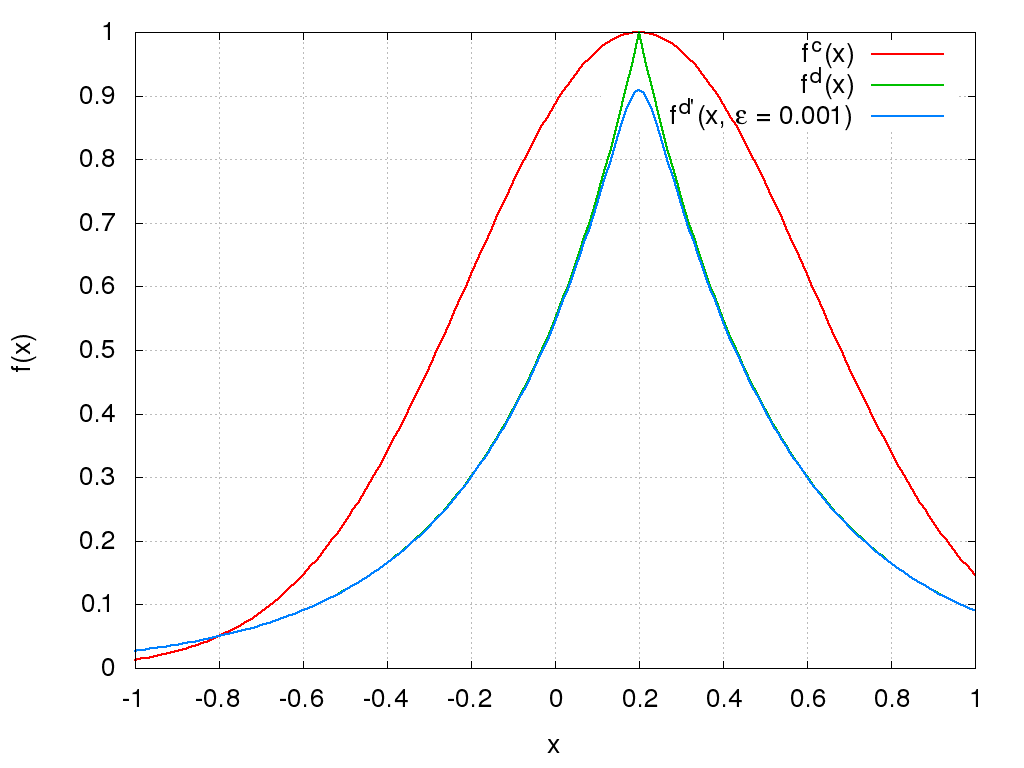
\includegraphics[scale=.2]{../pictures/gaussian_1D.png}
  \end{figure}

\end{minipage}





\end{frame}



%-------------------------------------------------------------------------------------
\begin{frame}{\bf Q-learning algoritmus - aproximácia}

Pre symetrické prechody medzi stavmi možno zjednodušiť na

\begin{align*}
f_j^1(\boldmath{s, a}) &= e^{ -\beta_{aj} \sum\limits_{i=1}^{n_s}{(s_i - \alpha_{aji})^2} }  \\
f_j^2(\boldmath{s, a}) &= \frac{1}{1 + {\beta_{aj} \sum\limits_{i=1}^{n_s}(s_i - \alpha_{aji})^2}}  \\
\end{align*}

a ich lineárna kombinácia

\begin{align}
    Q^x(s, a)&= \sum\limits_{j=1}^{l}w_{j a}f^x_{j}(s, a) \nonumber
\end{align}

kde $l$ je počet bázických funkcií a $x$ je voľba typu bázickej funkcie.



\end{frame}



%-------------------------------------------------------------------------------------
\begin{frame}{\bf Bloková schéma syntézy testovaného riešenia}

\begin{figure}[!htb]
\centering
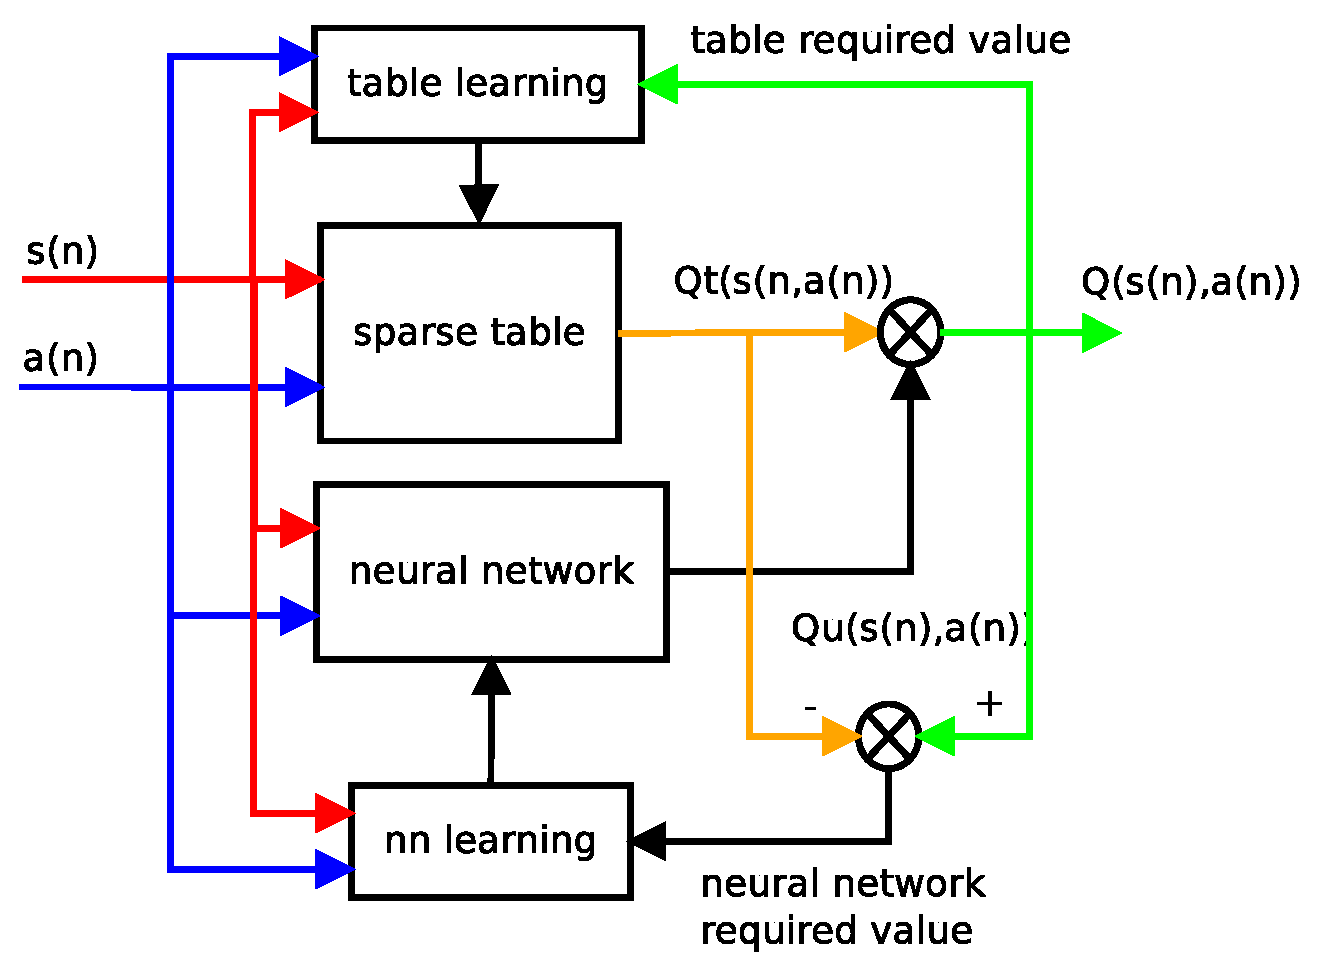
\includegraphics[scale=.4]{../diagrams/q_learning_hybrid.eps}
\end{figure}

\end{frame}

%-------------------------------------------------------------------------------------
\begin{frame}{\bf Schéma priebehu experimentov}

\begin{figure}[!htb]
\centering
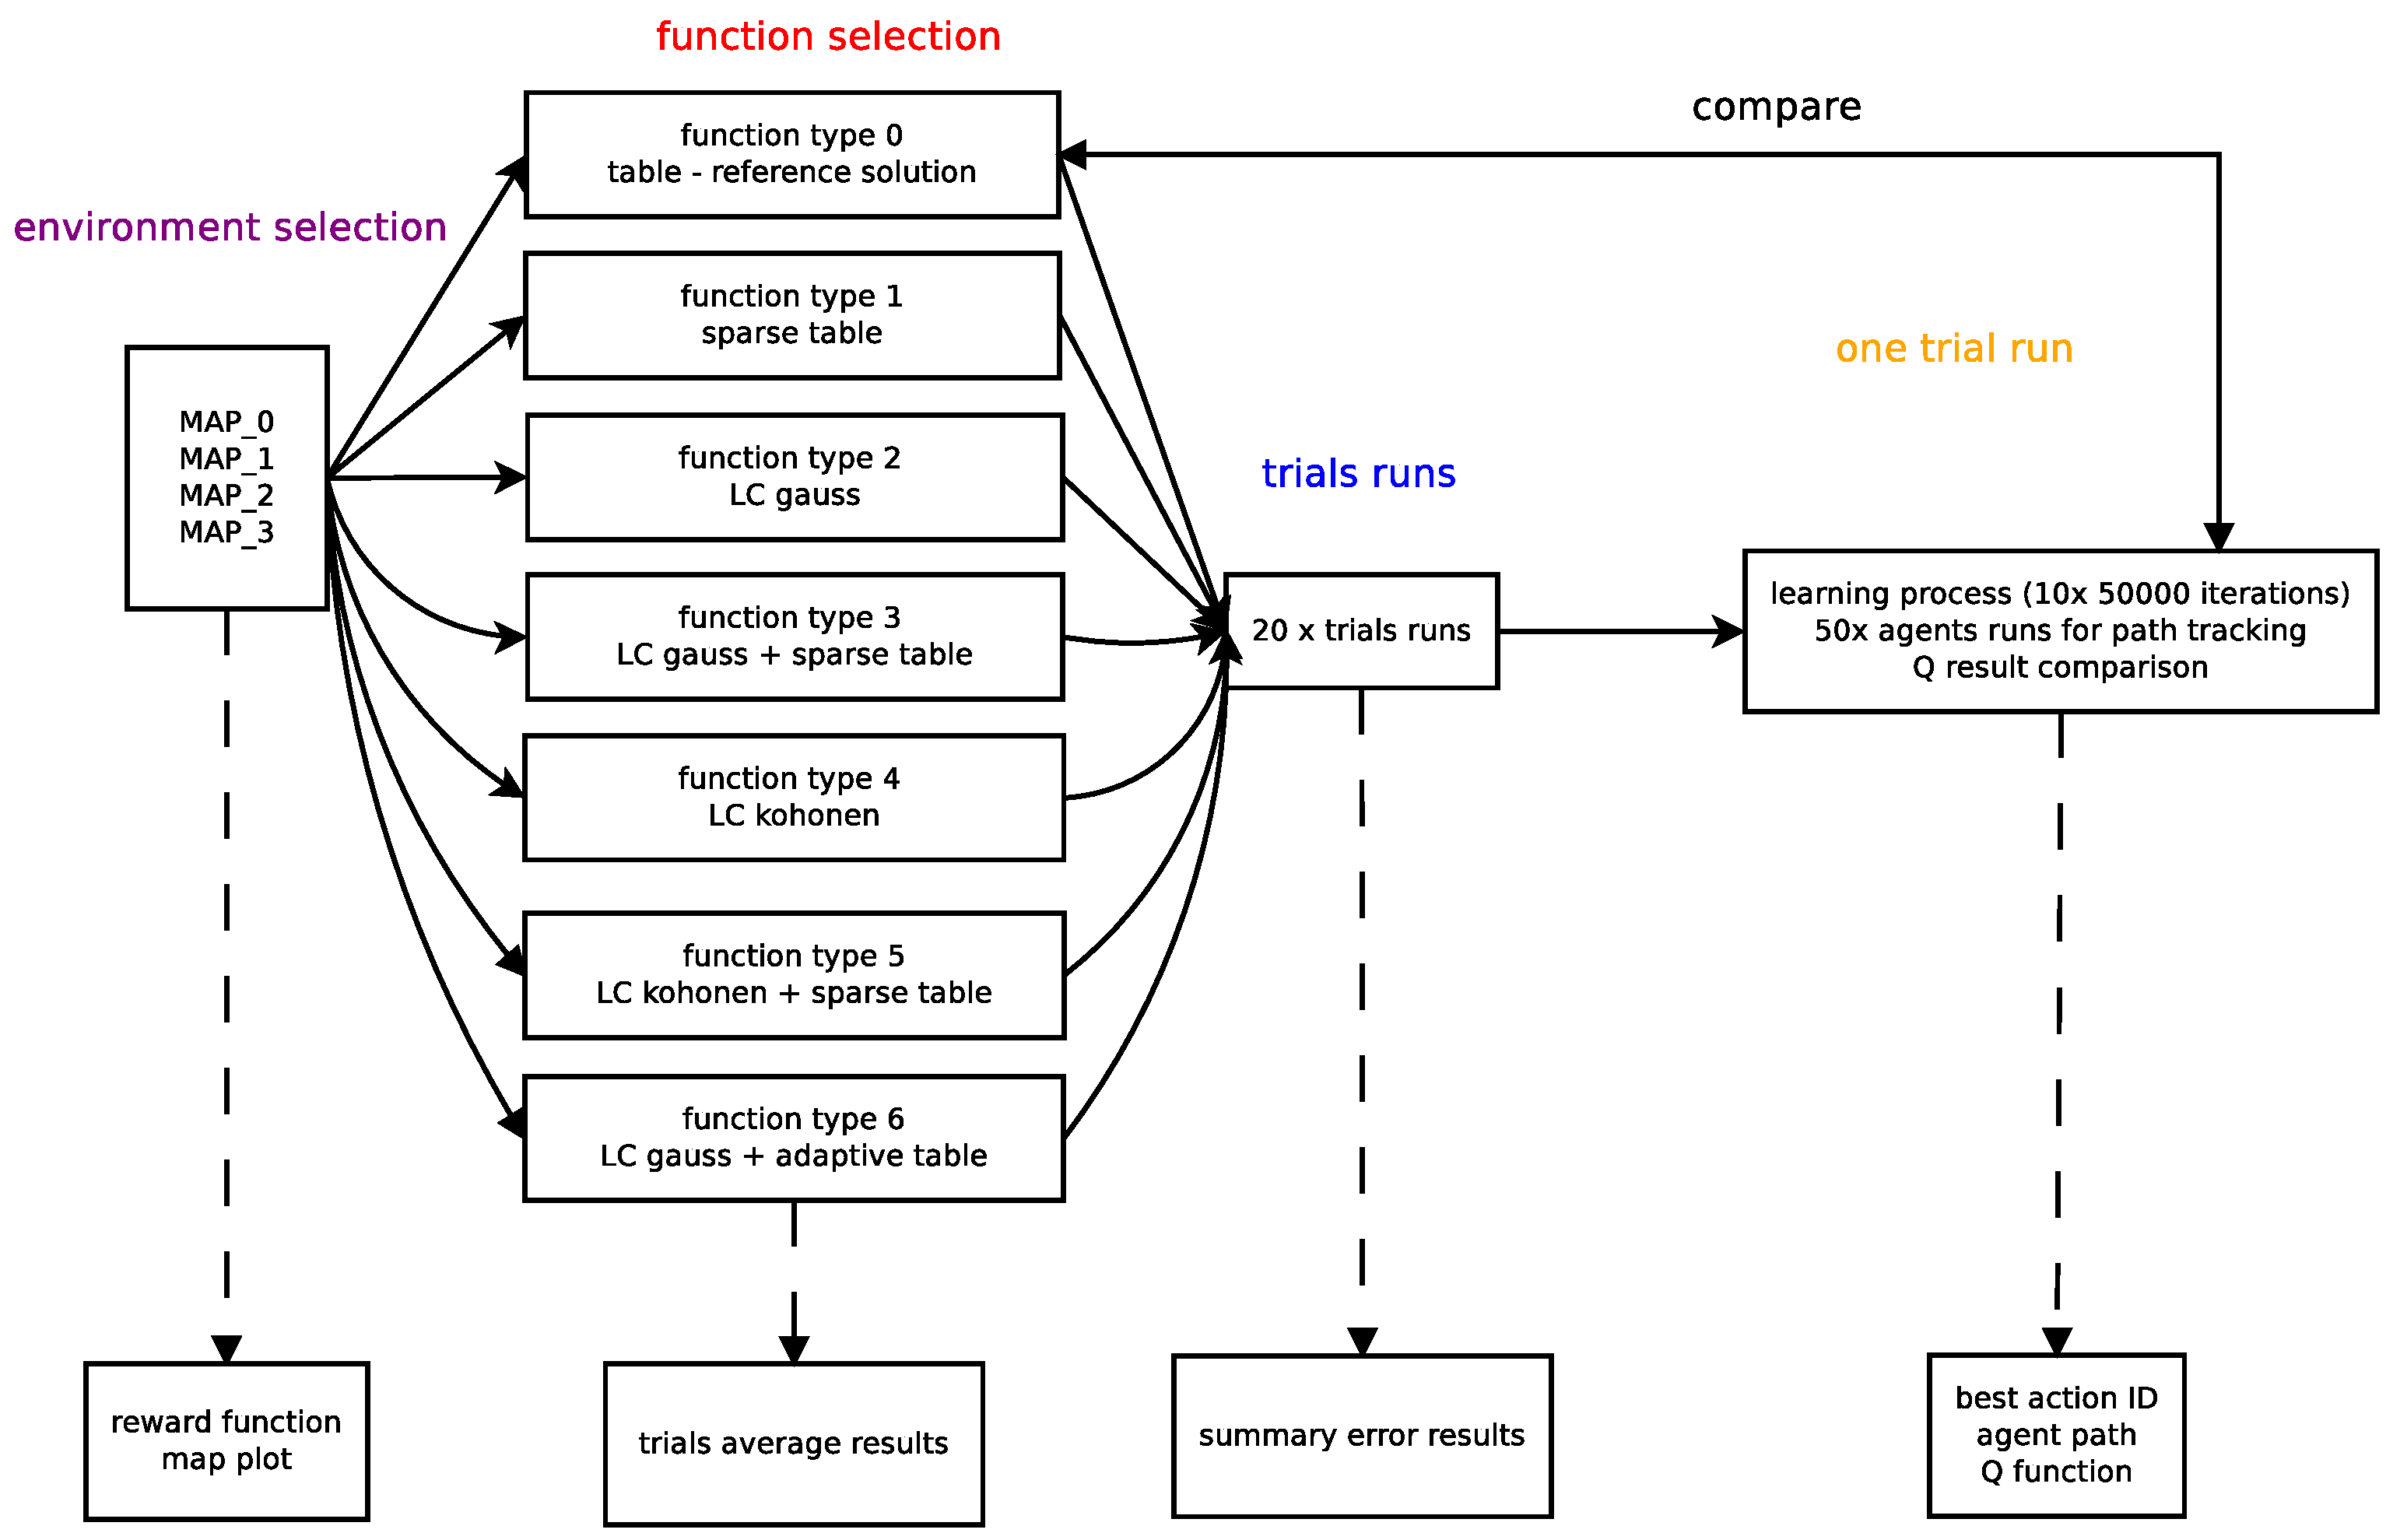
\includegraphics[scale=.22]{../diagrams/experiment_map_q_learning.eps}
\end{figure}

\end{frame}





%-------------------------------------------------------------------------------------
\begin{frame}{\bf Návrh experimentov - podmienky}

\begin{itemize}
\item 50000 iterácií učenia
\item rozmer $s$ je $n_s = 2$, rozmer $a$ je $n_a = 2$
\item predpis funkcie ohodnotení
\begin{align}
&Q(s(n),a(n)) = \nonumber \\
&\alpha Q(s(n-1),a(n-1)) \nonumber \\
&(1- \alpha)(R(s(n),a(n)) + \gamma \max_{a(n-1) \in \mathbb{A}} Q(s(n-1), a(n-1)) \nonumber
\end{align}

\item $R(s(n), a(n)) \in \langle -1, 1 \rangle$ náhodná mapa s 1 cieľovým stavom
\item $\gamma = 0.98$ a $\alpha = 0.7$
\item hustota referenčného riešenia = 1/32  (4096 stavov)
\item počet akcií v každom stave = 8
\item hustota riedkej tabuľky = 1/8  (1:16 pomer)
\item počet bázických funkcií $l = 64$
\item rozsah parametrov
    \begin{itemize}
      \item $\alpha_{ja}(n) \in \langle -1, 1 \rangle$
      \item $\beta_{ja}(n) \in \langle 0, 200 \rangle$
      \item $w_{ja}(n) \in \langle -4, 4 \rangle$
    \end{itemize}
\end{itemize}

\end{frame}


%-------------------------------------------------------------------------------------
\begin{frame}{\bf Návrh experimentov - podmienky}

$Q_{rt}(s(n),a(n))$ referenčná funkcia Q (funkcia 0), kde $t \in \langle 0, 19 \rangle $ je číslo trialu  \\
$Q_{jt}(s(n),a(n))$ testované funkcie Q a $j \in \langle 1, 5 \rangle $. \\

Celková chyba behu trialu $t$ je \\
\begin{equation}
e_{jt} = \sum\limits_{s, a}{(Q_{rt}(s,a) - Q_{jt}(s,a))^2}  \nonumber
\end{equation}

priemerná, minimálna, maximálna chyba a smerodatná odchylka \\
\begin{align}
\bar{a_j} &= \frac{1}{20}\sum\limits_{t}{e_{jt}}  \nonumber \\
{e^{min}_j} &= \min_{t}{e_{jt}}  \nonumber \\
{e^{max}_j} &= \max_{t}{e_{jt}}  \nonumber \\
{\sigma_j}^2 &= \frac{1}{20}\sum\limits_{t}{(\bar{a_j} - e_{jt})^2}  \nonumber
\end{align}

\end{frame}


%-------------------------------------------------------------------------------------
\begin{frame}{\bf Funkcia R(s, a), mapa 1 - Výsledky experimentov}
pre každý stav je zvolená rovnaka množina akcií. \\
Ďalej platí $s = (s[0], s[1])$.

\begin{figure}[!htb]
\centering
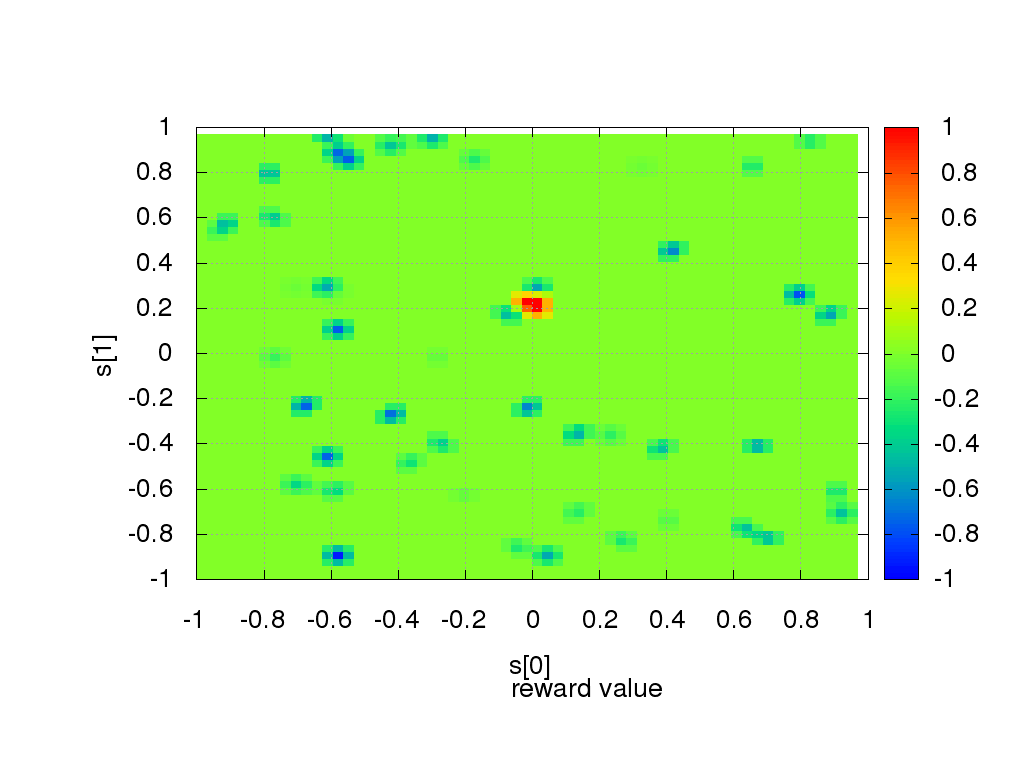
\includegraphics[scale=.4]{../../results_q_learning/map_1/reward_value_surface.png}
\end{figure}

\end{frame}



%-------------------------------------------------------------------------------------
\begin{frame}{\bf Mapa najlepších akcií - Výsledky experimentov}

Funkcia voľby najlepšej z 8 akcií v stave  $s = (s[0], s[1])$.

\begin{minipage}{.5\textwidth}

\begin{figure}[!htb]
\centering
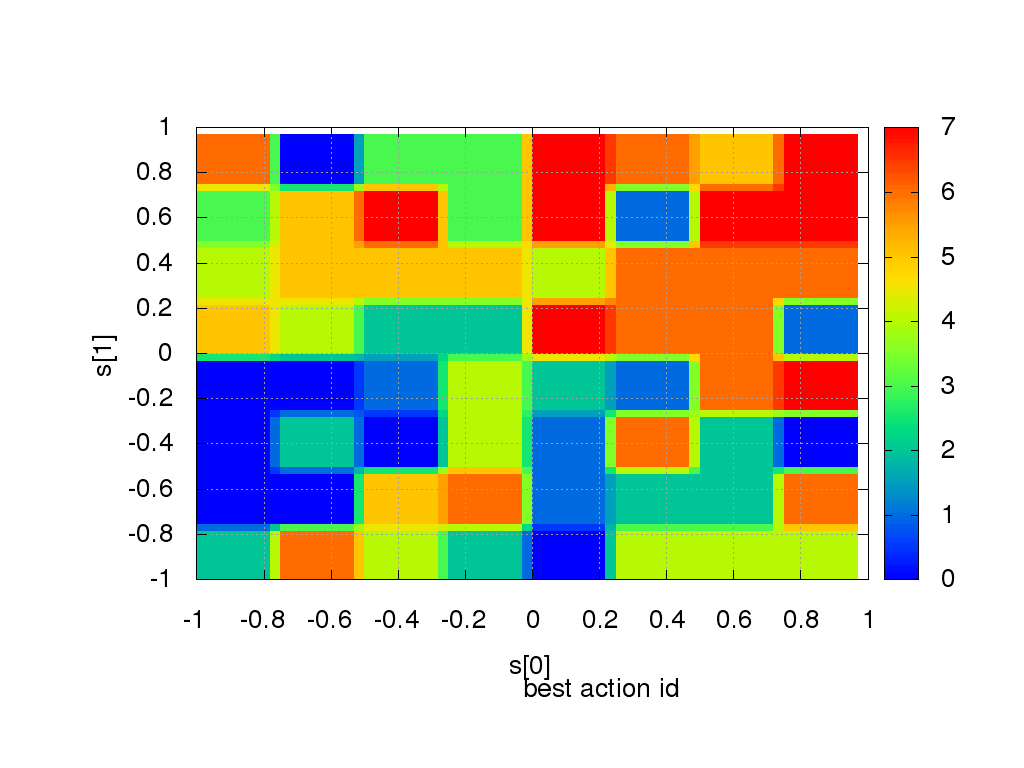
\includegraphics[scale=.21]{../../results_q_learning/map_1/function_type_1/iterations_10/action_best_value_log_surface.png}
\caption{sparse table}
\end{figure}

\end{minipage}%
\begin{minipage}{.5\textwidth}

\begin{figure}[!htb]
\centering
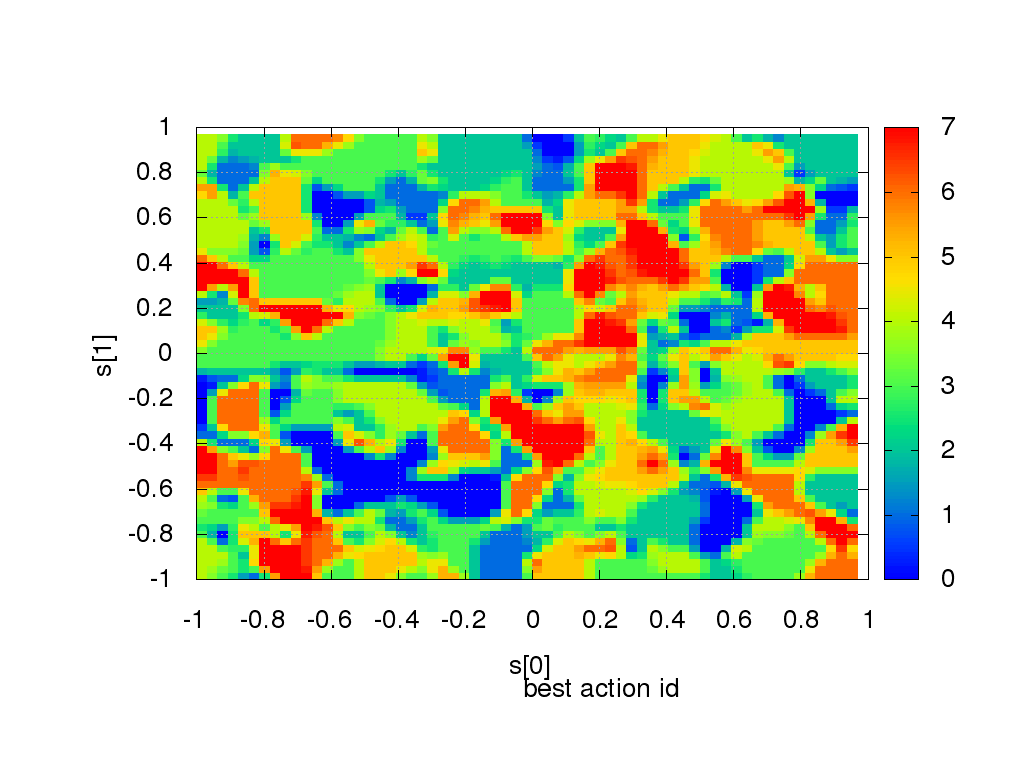
\includegraphics[scale=.21]{../../results_q_learning/map_1/function_type_2/iterations_10/action_best_value_log_surface.png}
\caption{linear combination Gauss}
\end{figure}


\end{minipage}
\end{frame}


%-------------------------------------------------------------------------------------
\begin{frame}{\bf Mapa najlepších akcií - Výsledky experimentov}

Funkcia voľby najlepšej z 8 akcií v stave  $s = (s[0], s[1])$.

\begin{minipage}{.5\textwidth}

\begin{figure}
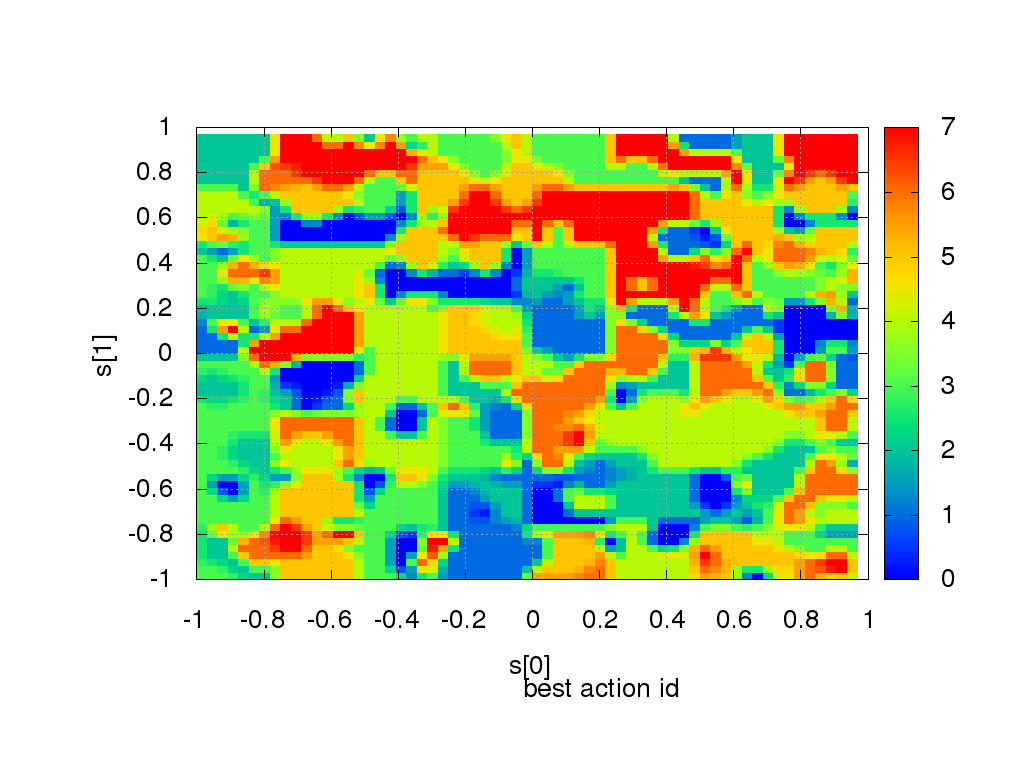
\includegraphics[scale=.21]{../../results_q_learning/map_1/function_type_3/iterations_10/action_best_value_log_surface.png}
\caption{sparse table + linear combination Gauss}
\end{figure}


\end{minipage}%
\begin{minipage}{.5\textwidth}

\begin{figure}
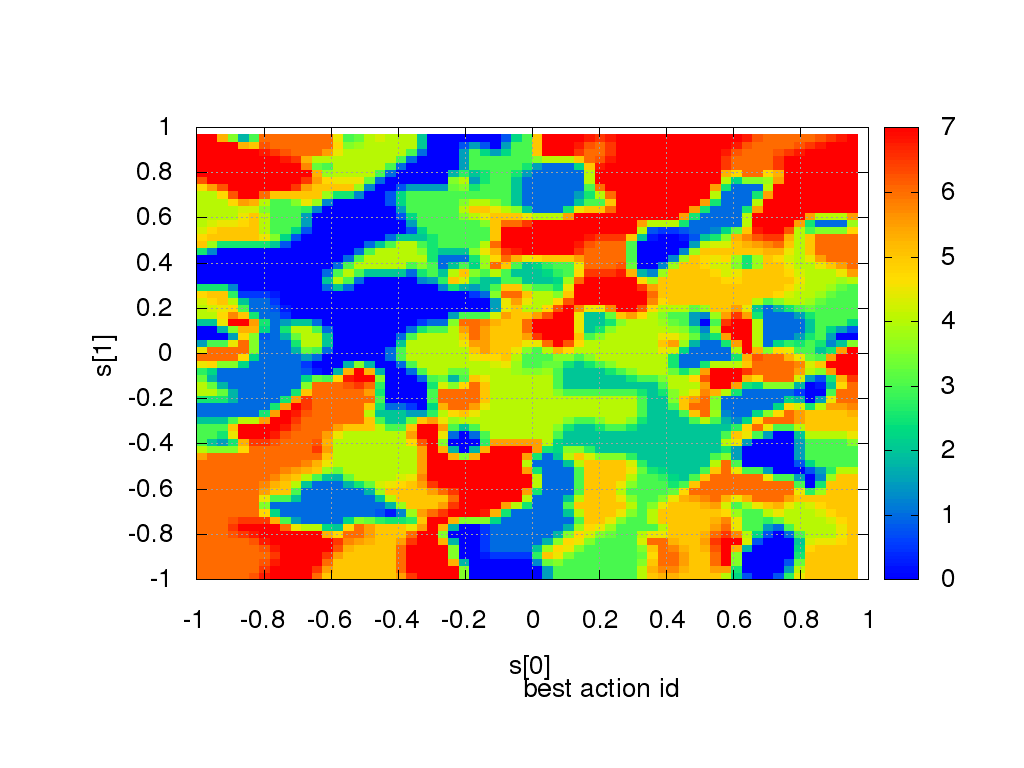
\includegraphics[scale=.21]{../../results_q_learning/map_1/function_type_4/iterations_10/action_best_value_log_surface.png}
\caption{linear combination Kohonen function}
\end{figure}


\end{minipage}
\end{frame}










%-------------------------------------------------------------------------------------
\begin{frame}{\bf Chybové funkcie - Výsledky experimentov}

\begin{equation}
e_{jt}(s) = (Q_{rt}(s,a - Q_{jt}(s,a))^2  \nonumber
\end{equation}

\begin{minipage}{.5\textwidth}

\begin{figure}[!htb]
\centering
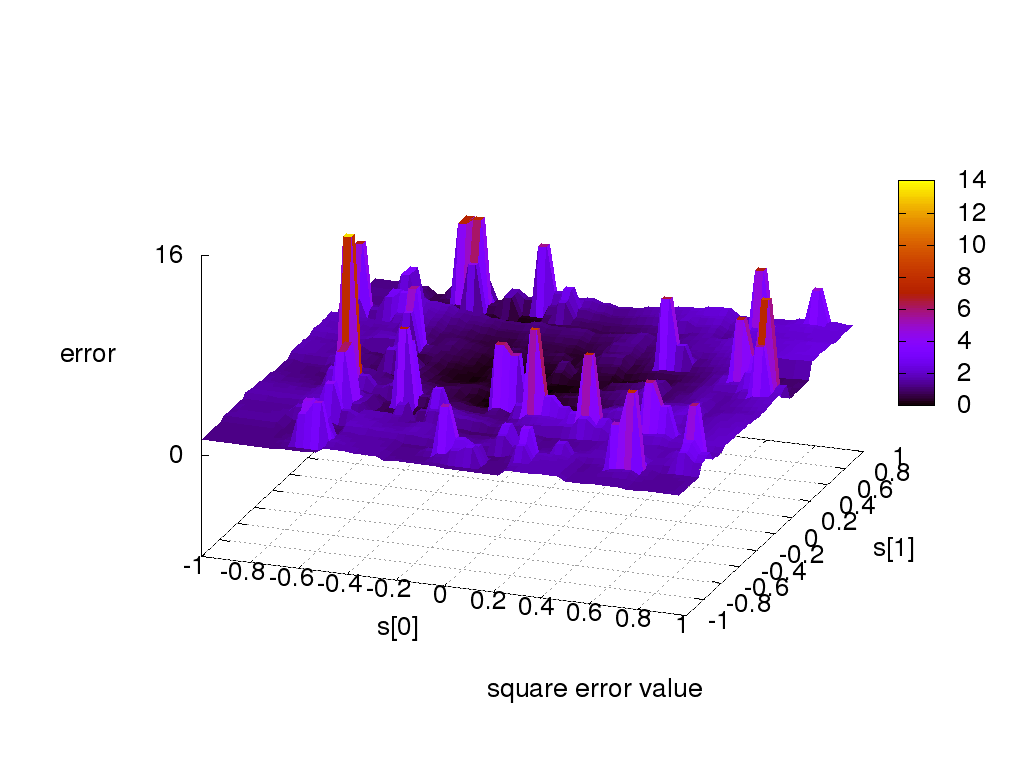
\includegraphics[scale=.2]{../../results_q_learning/map_1/function_type_1/q_learning_error.png}
\caption{sparse table}
\end{figure}

\end{minipage}%
\begin{minipage}{.5\textwidth}

\begin{figure}[!htb]
\centering
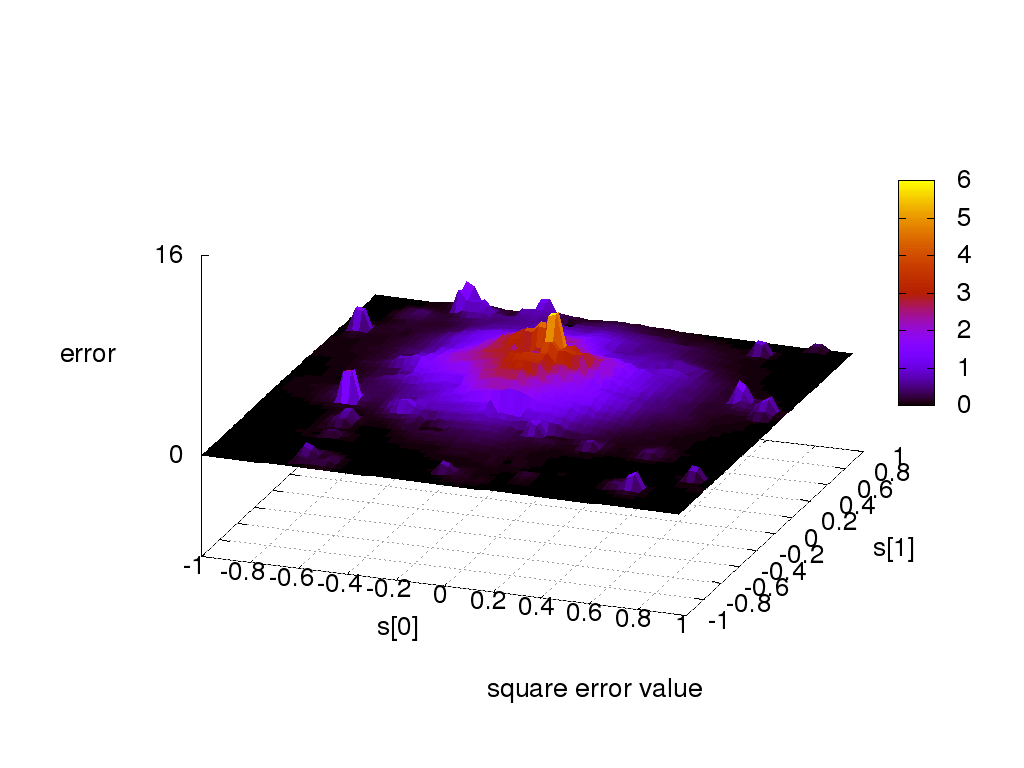
\includegraphics[scale=.2]{../../results_q_learning/map_1/function_type_2/q_learning_error.png}
\caption{linear combination Gauss}
\end{figure}


\end{minipage}
\end{frame}


%-------------------------------------------------------------------------------------
\begin{frame}{\bf Chybové funkcie - Výsledky experimentov}

\begin{equation}
e_{jt}(s) = (Q_{rt}(s,a - Q_{jt}(s,a))^2  \nonumber
\end{equation}

\begin{minipage}{.5\textwidth}

\begin{figure}[!htb]
\centering
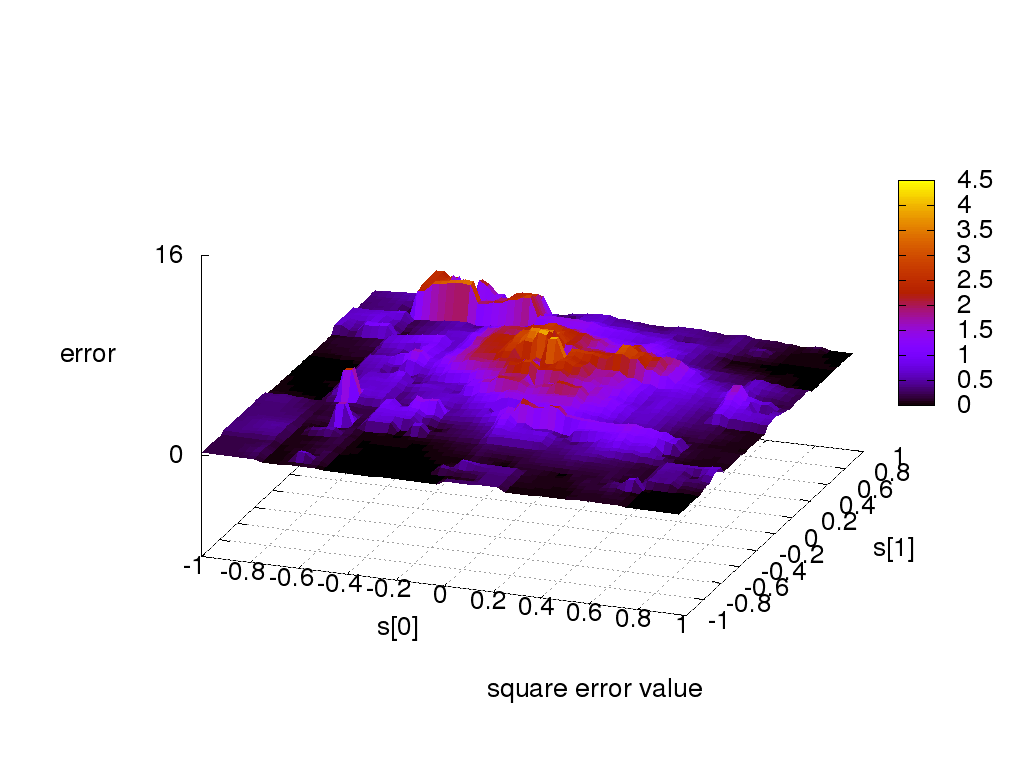
\includegraphics[scale=.2]{../../results_q_learning/map_1/function_type_3/q_learning_error.png}
\caption{sparse table + linear combination Gauss}
\end{figure}


\end{minipage}%
\begin{minipage}{.5\textwidth}

\begin{figure}[!htb]
\centering
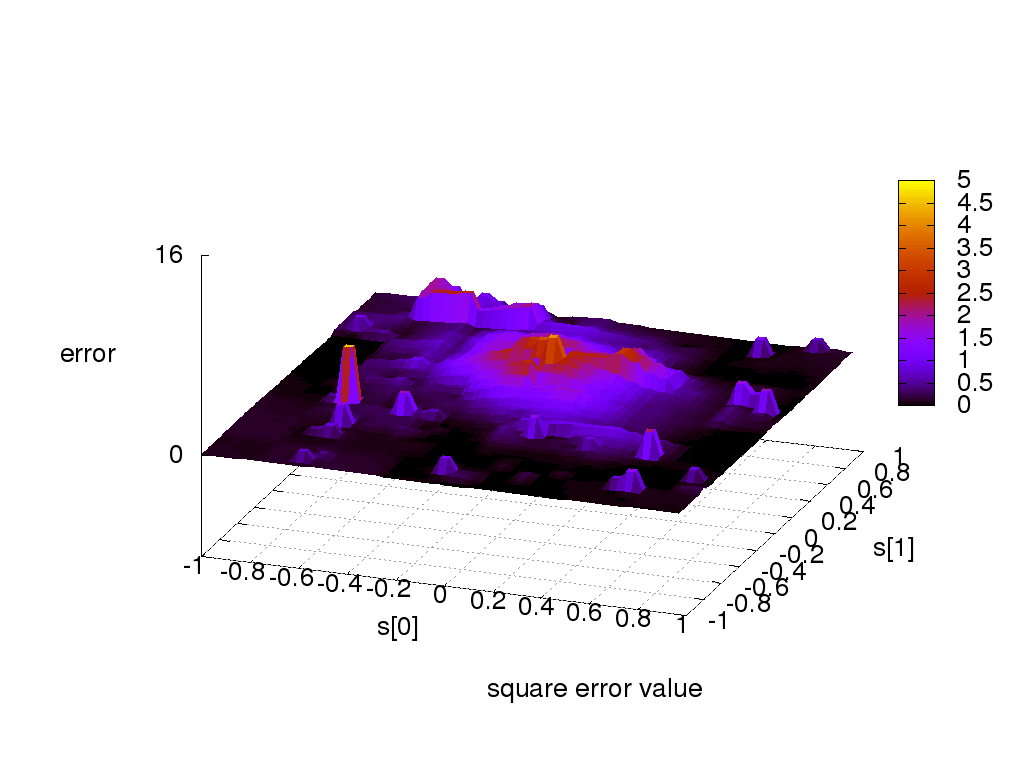
\includegraphics[scale=.2]{../../results_q_learning/map_1/function_type_4/q_learning_error.png}
\caption{linear combination Kohonen function}
\end{figure}


\end{minipage}
\end{frame}





%-------------------------------------------------------------------------------------
\begin{frame}{\bf max Q(s, a) - Výsledky experimentov}

\begin{minipage}{.5\textwidth}

\begin{figure}[!htb]
\centering
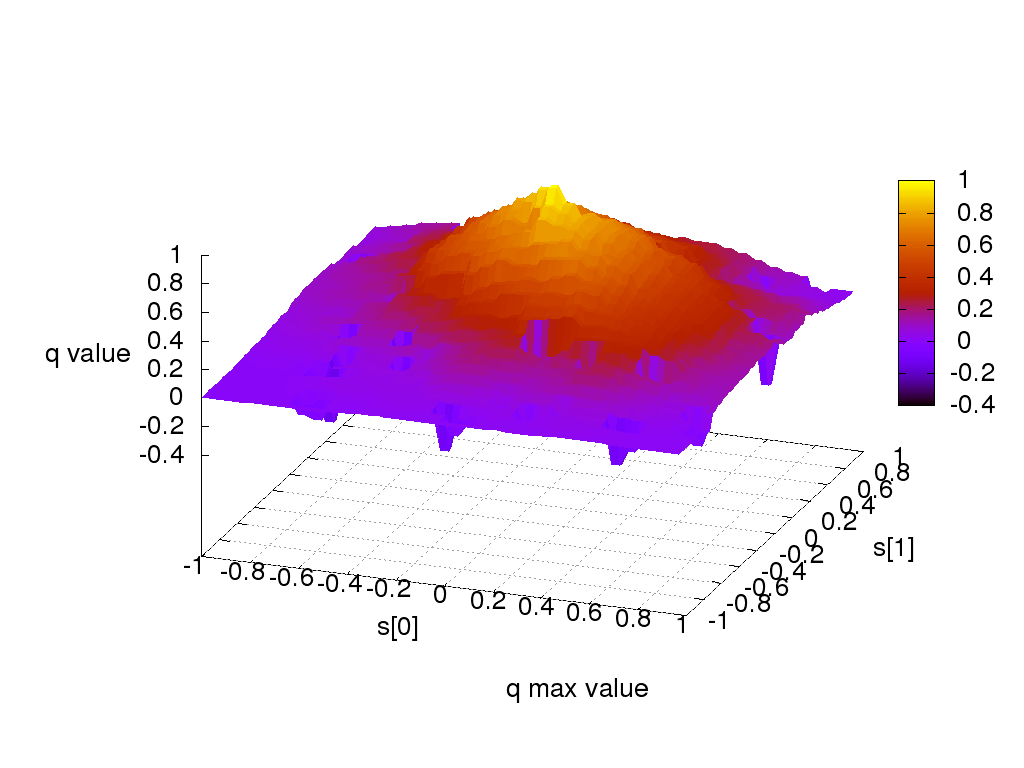
\includegraphics[scale=.2]{../../results_q_learning/map_1/function_type_0/iterations_10/q_learning_result.png}
\caption{reference table}
\end{figure}

\end{minipage}%
\begin{minipage}{.5\textwidth}

\begin{figure}[!htb]
\centering
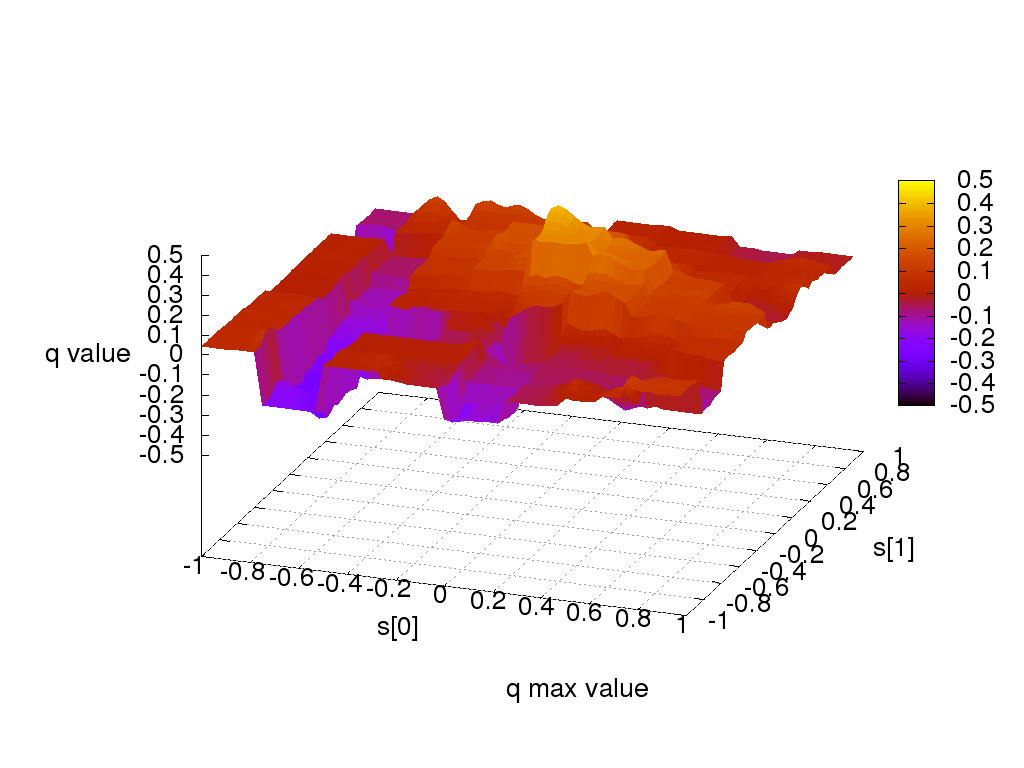
\includegraphics[scale=.2]{../../results_q_learning/map_1/function_type_3/iterations_10/q_learning_result.png}
\caption{sparse table + linear combination Gauss}
\end{figure}


\end{minipage}
\end{frame}



%-------------------------------------------------------------------------------------
\begin{frame}{\bf Priebeh trialov - Výsledky experimentov}

\begin{figure}[!htb]
\centering
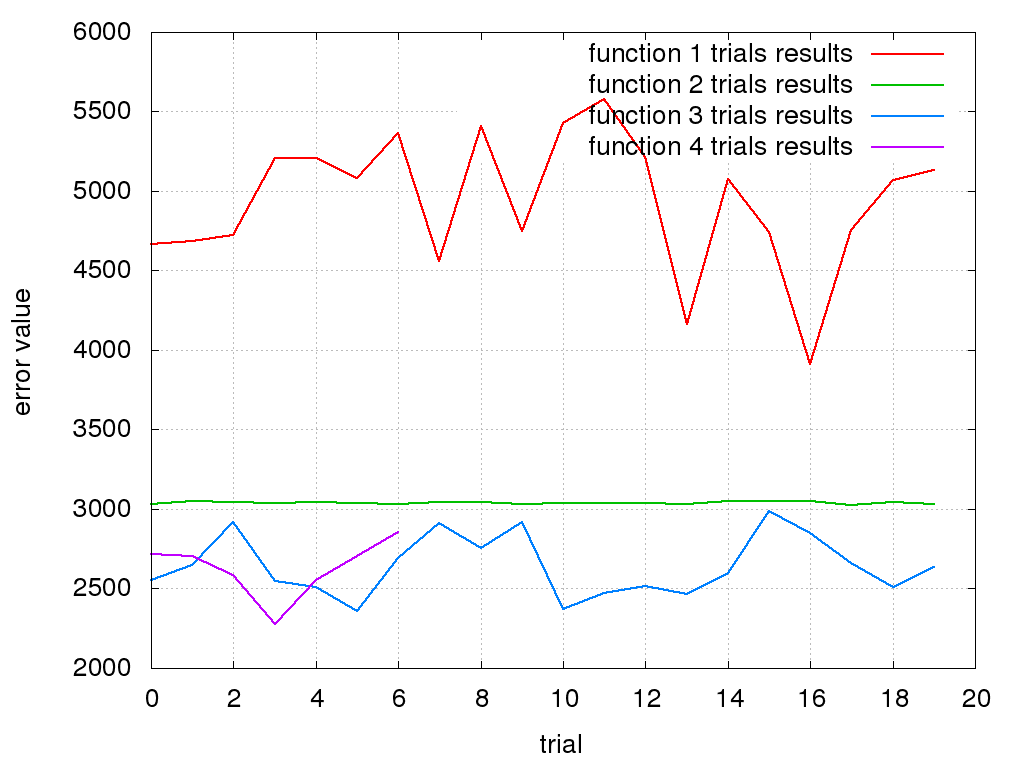
\includegraphics[scale=.36]{../../results_q_learning/map_1/trials_average_results_progress.png}
\end{figure}

\end{frame}



%-------------------------------------------------------------------------------------
\begin{frame}{\bf Mapa 1 - Výsledky experimentov}

\begin{figure}[!htb]
\centering
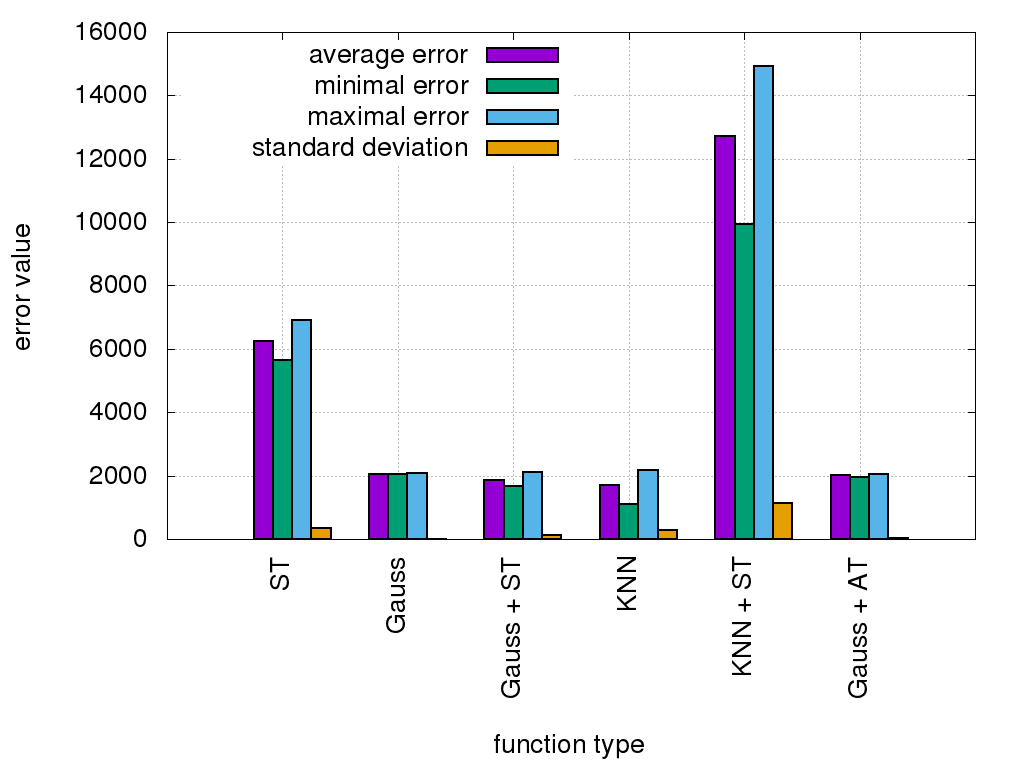
\includegraphics[scale=.36]{../../results_q_learning/map_1/trials_average_results.png}
\end{figure}

\end{frame}


%-------------------------------------------------------------------------------------
\begin{frame}{\bf Mapa 0 - Výsledky experimentov}

\begin{figure}[!htb]
\centering
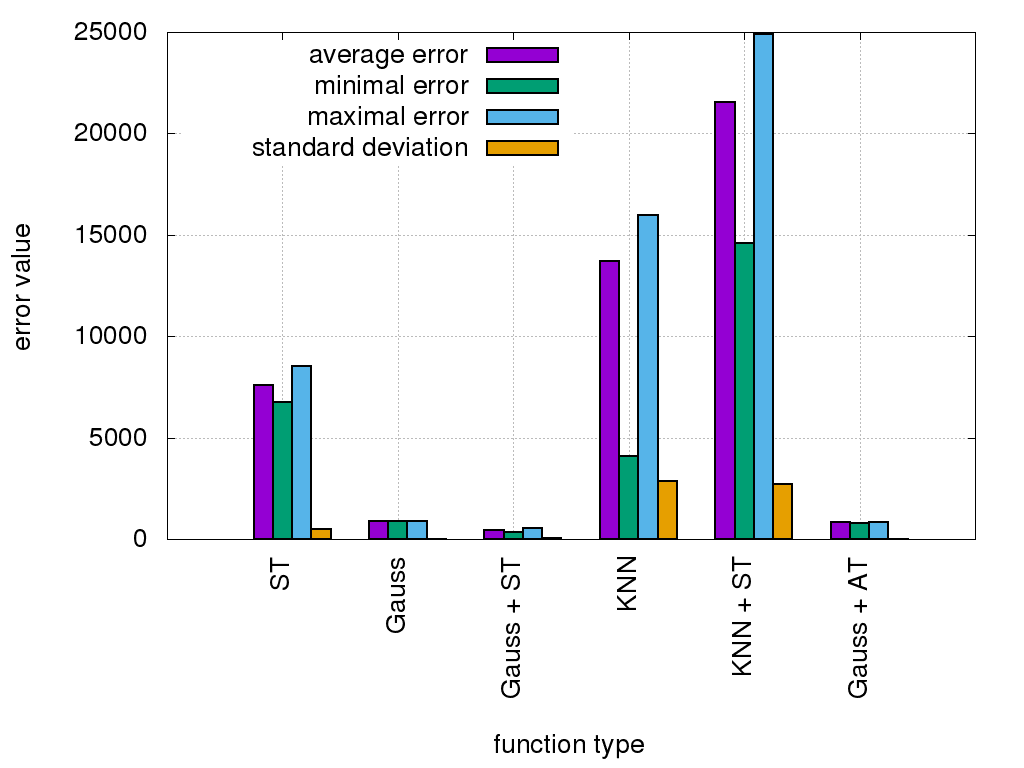
\includegraphics[scale=.36]{../../results_q_learning/map_0/trials_average_results.png}
\end{figure}

\end{frame}

%-------------------------------------------------------------------------------------
\begin{frame}{\bf Mapa 2 - Výsledky experimentov}

\begin{figure}[!htb]
\centering
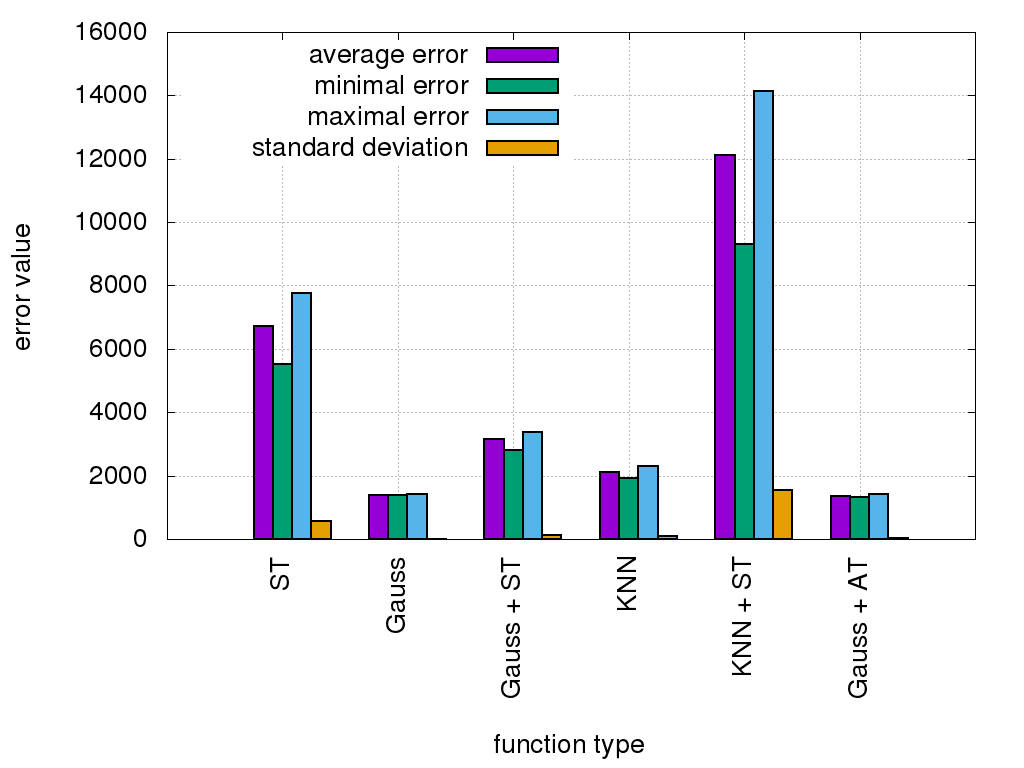
\includegraphics[scale=.36]{../../results_q_learning/map_2/trials_average_results.png}
\end{figure}

\end{frame}

%-------------------------------------------------------------------------------------
\begin{frame}{\bf Mapa 3 - Výsledky experimentov}

\begin{figure}[!htb]
\centering
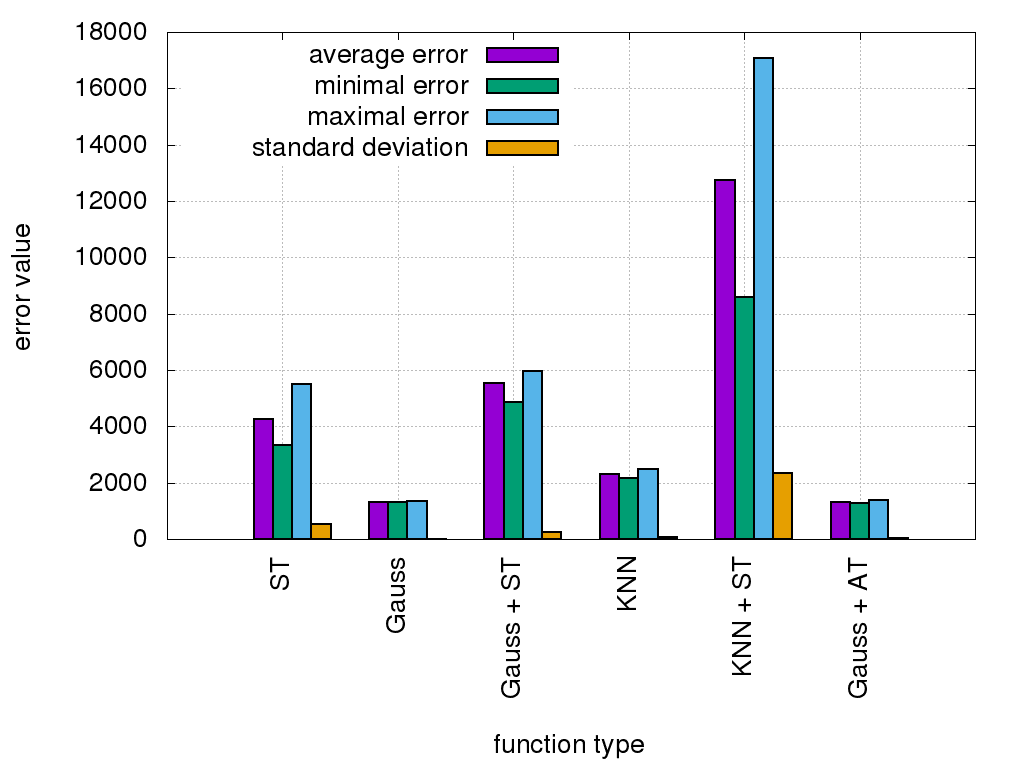
\includegraphics[scale=.36]{../../results_q_learning/map_3/trials_average_results.png}
\end{figure}

\end{frame}

%-------------------------------------------------------------------------------------
\begin{frame}{\bf Ďakujem za pozornosť}

\centerline{michal.chovanec@yandex.ru}
\centerline{https://github.com/michalnand/q\_learning}

\begin{figure}[!htb]
\centering
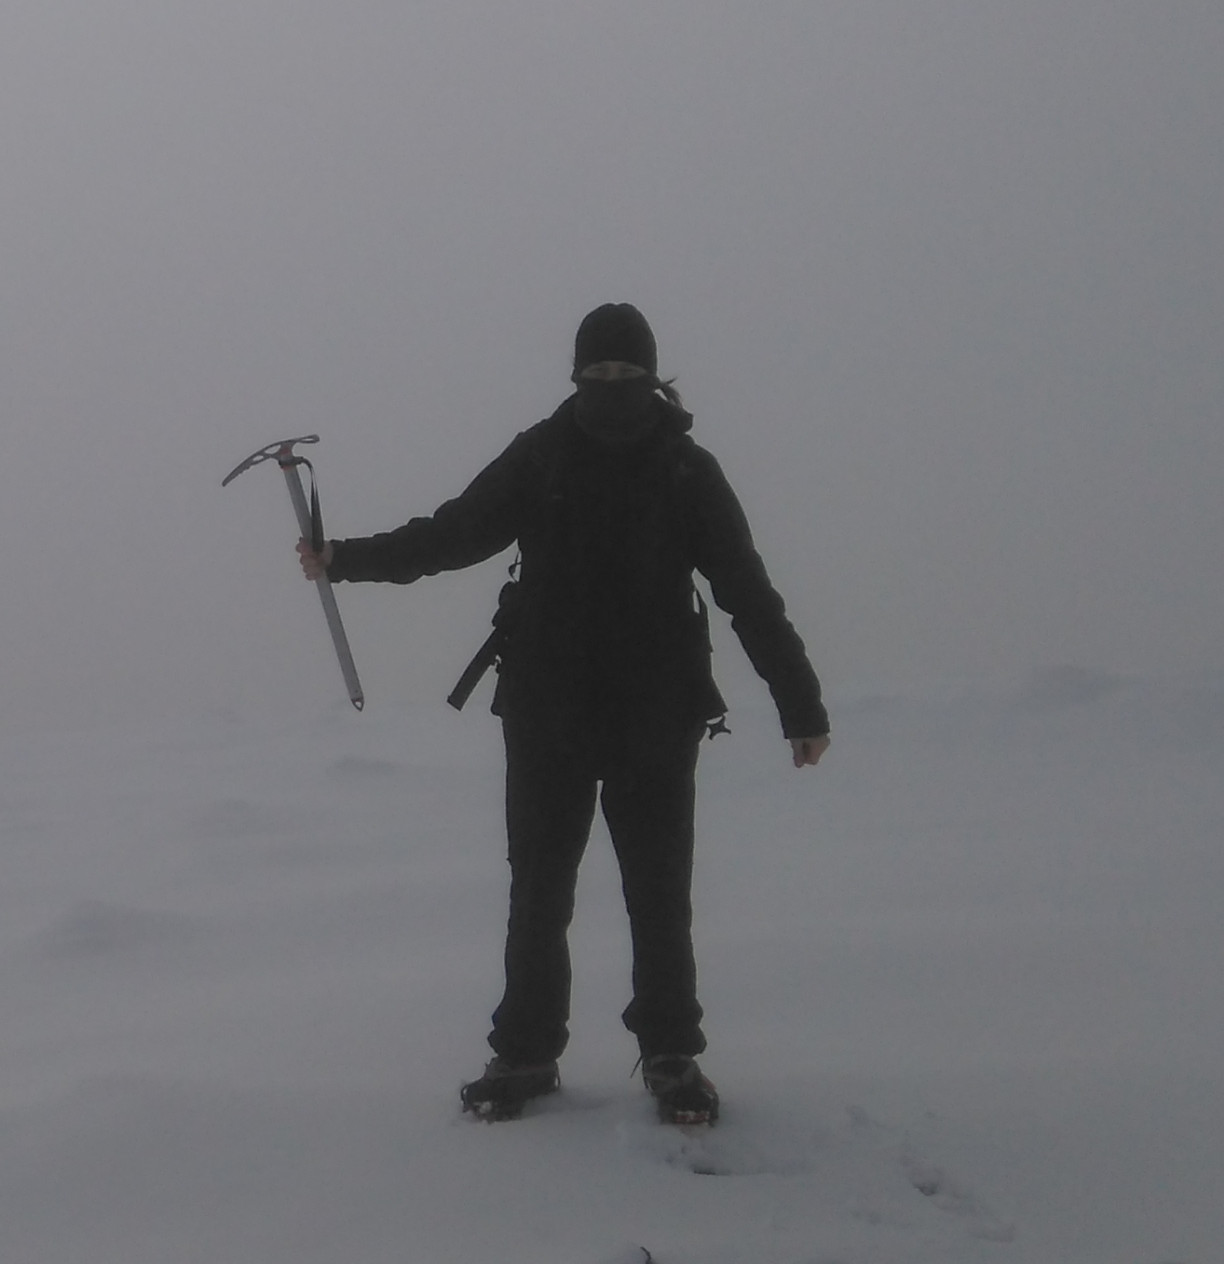
\includegraphics[scale=.15]{../pictures/me.jpg}
\end{figure}



\end{frame}

\end{document}
